\documentclass[11pt,a4paper]{article}
\usepackage[T1]{fontenc}
\usepackage[utf8]{inputenc}
\usepackage{lmodern}
\usepackage[margin=2.3cm]{geometry}
\usepackage{amsmath,amssymb}
\usepackage{booktabs}
\usepackage{graphicx}
\usepackage{siunitx}
\usepackage{float}
\usepackage{enumitem}
\usepackage{xcolor}
\usepackage[font=small,labelfont=bf]{caption}
\usepackage{microtype}
\usepackage{cite}
\usepackage[colorlinks=true,linkcolor=black,urlcolor=blue!50!black,citecolor=black]{hyperref}
\graphicspath{{figures/}}
\sisetup{exponent-product=\cdot}
\setlist{itemsep=2pt,topsep=4pt}
\newcommand{\LL}{\Lambda_L}
\newcommand{\LH}{\Lambda_H}
\newcommand{\weff}{w_\mathrm{eff}}
\newcommand{\ws}{w^{*}}
\newcommand{\wt}{w_t}
\newcommand{\M}{\textsuperscript{[M]}}
\newcommand{\Hd}{\textsuperscript{[H]}}
\newcommand{\As}{\textsuperscript{[A]}}
\newcommand{\cymm}{\,cy/mm}
\newcommand{\code}[1]{\texttt{#1}}

\title{Recombination of dual-energy CEM images of the L2 phantom:\\ Siemens' weighting as measured from its images,\\ and the tuned recombination\\[4pt]
\large Method documentation for \code{l2\_tuned\_recombination.py}\\ and its multi-system version (Siemens and Hologic)}
\author{Working document for the thesis}
\date{18 November 2026 (revised 19 November 2026)}

\begin{document}
\maketitle

{\sloppy \noindent\textbf{Scope.} This document describes one method only: the one implemented in the script
\code{l2\_tuned\_recombination.py}, which lies next to the measurements on the SanDisk, together with the
measurements that its fixed numbers come from. It covers (i) how Siemens' recombined image is built from the low- and high-energy images, as far as this can
be measured from the images themselves, (ii) how the amount of background structure that Siemens' recombination
leaves in real breasts was measured, and (iii) how the L2 phantom images are recombined so that the same amount is
left. Section~\ref{sec:hologic} applies the same method, with \code{l2\_tuned\_recombination\_multisystem.py}, to
images of the phantom from a Hologic Selenia Dimensions and compares the two systems. Earlier trials that are not
part of the scripts are left out.\par}

\medskip
\noindent\textbf{How statements are marked.}
\M\ measured in this work from the images; \Hd\ read from the DICOM header; \As\ an assumption.
Siemens does not publish its algorithm. Everything said here about Siemens' processing is a description of what its
images contain, not of its code.

\medskip
\noindent\textbf{Patient data.} The breast numbers are spectra averaged over regions and views. No patient image, name,
date or identifier is part of this document or of the script.

\tableofcontents
\newpage

% =====================================================================================================================
\section{Data and notation}

\subsection{Images}
Each contrast-enhanced mammography (CEM) exposure of the system consists of three DICOM images\Hd:
\begin{center}\small
\begin{tabular}{llll}
\toprule
 & low energy (LE) & high energy (HE) & recombined ($R$) \\
\midrule
ImageType & \code{LOW\_ENERGY} & \code{HIGH\_ENERGY} & \code{RECOMBINED, SUBTRACTION} \\
presentation intent & for processing & for processing & for presentation \\
tube voltage, anode/filter & 28--32 kV, W/Rh & 49 kV, W/Ti & -- \\
stored bits & 14 & 14 & 12 \\
relationship to exposure & linear, sign $+1$ & linear, sign $+1$ & sign $-1$ \\
display window & -- & -- & centre 2600, width 2100 \\
\bottomrule
\end{tabular}
\end{center}
System: Siemens MAMMOMAT Revelation, software VC20G, detector LV2-33695, pixel pitch $p=\SI{0.085}{mm}$, image size
$3518\times2800$ pixels, anti-scatter grid in\Hd. The three images of one exposure are paired by the irradiation-event
UIDs in their headers.

The phantom data are 112 exposures of the L2 phantom (July 2026), compressed thickness 53--55 mm, at three LE tube
voltages and three exposure levels (Table~\ref{tab:data}). The HE exposure is always 49 kV.

\begin{table}[H]\centering\small
\caption{The L2 exposures processed by the script (all that were found on the drive). mAs: median of the group.
$W$: Siemens' weight as written in the header of the recombined image (Section~\ref{sec:header}).}\label{tab:data}
\begin{tabular}{llrrrl}
\toprule
LE kV & level & exposures & LE mAs & HE mAs & header $W$ \\
\midrule
28 & low    & 12 & 130 & 28.8 & 0.255 (0.254 at 53 mm) \\
28 & normal & 12 & 161 & 34.8 & 0.255 \\
28 & high   & 12 & 201 & 42.0 & 0.255 \\
29 & (one stray exposure) & 1 & 180 & 37.6 & 0.258 \\
30 & low    & 13 & 100 & 29.0 & 0.265 \\
30 & normal & 12 & 122 & 35.0 & 0.265 \\
30 & high   & 14 & 153 & 42.5 & 0.265 (0.266 at 55 mm) \\
32 & low    & 12 & 76  & 29.1 & 0.293 \\
32 & normal & 12 & 92  & 34.8 & 0.293 (0.292 at 53 mm) \\
32 & high   & 12 & 113 & 42.7 & 0.293 \\
\bottomrule
\end{tabular}
\end{table}
\noindent Two of the 30 kV exposures were made with the paddle not lowered (thickness 137--138 mm in the header,
$W=0.285$). The script processes them like the others; they are not used in the reader study.

\subsection{Log signal}
The stored value $I$ of the LE and HE images is proportional to the detector exposure\Hd. The method works on the
log signal
\begin{equation}
\Lambda(x,y) = -\ln I(x,y), \qquad I \text{ clipped at } 1 \text{ from below.}
\label{eq:log}
\end{equation}
For a narrow beam through materials $i$ of thickness $t_i$, $I = I_0\exp(-\sum_i \mu_i t_i)$, so
$\Lambda = \sum_i \mu_i t_i - \ln I_0$: the log signal is linear in the material thicknesses, and a local change of
thickness $\Delta t$ of material $a$ replaced by material $b$ changes it by $\Delta\Lambda=(\mu_a-\mu_b)\,\Delta t$.
This is the basis of dual-energy and contrast-enhanced subtraction imaging \cite{lehmann1981,lewin2003,korporaal2018}.
$\LL$ and $\LH$ denote the log signals of the LE and the HE image. A possible constant offset of the stored
values is not corrected (it is not known for this unit)\As.

\subsection{Weighted subtraction and the cancelling weight}
If the object consists of two background materials (in the phantom: spheres and the liquid around them; in the
breast: glandular and adipose tissue), the structure in both log images comes from the same thickness map
$\tau(x,y)$:
\begin{equation}
\LL \simeq \Delta\mu_L\,\tau + \ldots,\qquad \LH \simeq \Delta\mu_H\,\tau + \ldots
\end{equation}
The weighted difference
\begin{equation}
D_w = \LH - w\,\LL
\label{eq:Dw}
\end{equation}
then contains the structure with the factor $(\Delta\mu_H - w\,\Delta\mu_L)$. It vanishes for
$w=\Delta\mu_H/\Delta\mu_L$, the \emph{cancelling weight} of that material pair \cite{alvarez1976,lehmann1981,johns1985}.
Iodine has a different ratio (its K-edge at 33.2 keV lies between the two spectra) and therefore stays in $D_w$
\cite{lewin2003,korporaal2018}. A weight that cancels breast tissue does not cancel another material pair
\cite{lehmann1981,johns1987}: this is the starting point of the whole work. The cancelling weight depends on the
spectra and on thickness and composition \cite{carton2010,hu2017}, and in clinical CEM the cancellation of breast
tissue is incomplete \cite{hill2013b}.

\subsection{Spatial-frequency bands and spectra}\label{sec:spectra}
All quantities are measured per spatial-frequency band in square regions of interest (ROIs) of $N=128$ pixels
(\SI{10.88}{mm}) placed on a grid with half overlap (step 64 pixels, \SI{5.44}{mm}). For an image $a$ and ROI $j$:
\begin{enumerate}
\item \emph{Detrend.} A two-dimensional polynomial of second order
($1,x,y,x^2,y^2,xy$) is fitted to the ROI by least squares and subtracted. This removes level, gradient and curvature,
which would otherwise leak into the lowest bands. Subtracting a second-order polynomial was the best of four
detrending methods compared for noise-power-spectrum measurement in \cite{zhou2011}.
\item \emph{Window.} The result is multiplied by a separable Hann window $h[m,n]=h[m]\,h[n]$ \cite{harris1978}.
\item \emph{Transform.} $A_j(\mathbf k)=\sum_{m,n} h[m,n]\,a'_j[m,n]\,e^{-2\pi i(k_x m+k_y n)/N}$, with the frequency of
sample $\mathbf k$ equal to $|\mathbf f_{\mathbf k}|=\sqrt{k_x^2+k_y^2}\,/(Np)$; the frequency step is
$1/(Np)=\SI{0.0919}{cy/mm}$ and the Nyquist frequency \SI{5.88}{cy/mm}.
\end{enumerate}
The auto- and cross-spectral densities of two images $X$, $Y$ in band $b$ are the averages over the kept ROIs
$j=1\ldots J$ and over the DFT samples $\mathcal K_b$ whose radial frequency lies in the band:
\begin{equation}
S_{XY}(b)=\frac{p^2}{\sum_{m,n}h[m,n]^2}\;\frac{1}{J\,|\mathcal K_b|}\sum_{j=1}^{J}\sum_{\mathbf k\in\mathcal K_b}
\operatorname{Re}\!\big\{X_j(\mathbf k)\,\overline{Y_j(\mathbf k)}\big\}.
\label{eq:psd}
\end{equation}
For log signals $S$ has the unit mm$^2$; for the recombined image grey values$^2\,$mm$^2$. The six spectra used
are $S_{LL}$, $S_{HH}$, $S_{HL}$ (from $\LL$, $\LH$) and $S_{RH}$, $S_{RL}$, $S_{RR}$ (with the recombined image $R$).
This is the averaged, windowed periodogram (Welch's method \cite{welch1967}) applied to two-dimensional ROIs; half
overlap is recommended with a Hann window \cite{carter1973}. The principle is that of noise-power-spectrum
measurement of x-ray detectors \cite{dobbins2006,iec62220}, but ROI size and window are not those of the IEC
procedure.

The thirteen bands and the number of DFT samples per ROI in each are listed in Table~\ref{tab:bands}. The band
centre is the geometric mean of its edges. The three lowest bands contain four samples each per ROI; with about 280
ROIs per image each band value rests on more than 1000 samples.

\begin{table}[H]\centering\small
\caption{Frequency bands, DFT samples per ROI, and the fixed per-band numbers of the script: the noise shape $g$
(Section~\ref{sec:noise}), Siemens' LE filter $K$ used for the breast target (Section~\ref{sec:siemensresults}), the
breast target $T$ and the total breast residual $P_D$ (Section~\ref{sec:breast}; mm$^2$).}\label{tab:bands}
\begin{tabular}{rrrrrrrr}
\toprule
band (cy/mm) & centre & samples & $g$ & $K$ & $T$ (median) & $P_D$ (median) & $P_D$ (lowest--highest) \\
\midrule
0.06--0.10 & 0.077 & 4    & 2.68 & 1.00  & \num{7.96e-6} & \num{1.03e-5} & \num{4.6e-6}--\num{2.5e-5} \\
0.10--0.15 & 0.122 & 4    & 2.65 & 1.01  & \num{1.10e-5} & \num{1.33e-5} & \num{5.5e-6}--\num{3.4e-5} \\
0.15--0.20 & 0.173 & 4    & 2.62 & 1.01  & \num{1.15e-5} & \num{1.37e-5} & \num{5.4e-6}--\num{2.7e-5} \\
0.20--0.30 & 0.245 & 24   & 2.58 & 0.98  & \num{8.16e-6} & \num{1.04e-5} & \num{4.2e-6}--\num{1.6e-5} \\
0.30--0.40 & 0.346 & 24   & 2.52 & 0.91  & \num{3.85e-6} & \num{6.01e-6} & \num{3.3e-6}--\num{1.0e-5} \\
0.40--0.60 & 0.490 & 76   & 2.43 & 0.81  & \num{1.80e-6} & \num{3.85e-6} & \num{2.8e-6}--\num{6.2e-6} \\
0.60--0.80 & 0.693 & 104  & 2.32 & 0.62  & \num{9.09e-7} & \num{2.84e-6} & \num{2.5e-6}--\num{3.5e-6} \\
0.80--1.00 & 0.894 & 132  & 2.21 & 0.43  & \num{3.78e-7} & \num{2.16e-6} & \num{2.0e-6}--\num{2.6e-6} \\
1.00--1.50 & 1.225 & 472  & 2.07 & 0.20  & 0 & \num{1.69e-6} & \num{1.5e-6}--\num{1.8e-6} \\
1.50--2.00 & 1.732 & 636  & 1.91 & 0.04  & 0 & \num{1.33e-6} & \num{1.2e-6}--\num{1.4e-6} \\
2.00--3.00 & 2.449 & 1860 & 1.69 & 0.00  & 0 & \num{1.12e-6} & \num{1.0e-6}--\num{1.2e-6} \\
3.00--4.00 & 3.464 & 2616 & 1.38 & 0.00  & 0 & \num{9.04e-7} & \num{8.3e-7}--\num{9.7e-7} \\
4.00--5.88 & 4.850 & 6884 & 1.00 & 0.01  & 0 & \num{6.04e-7} & \num{5.6e-7}--\num{6.7e-7} \\
\bottomrule
\end{tabular}
\end{table}

\subsection{Coherence and the cancelling weight per band}
For each band the weight that minimises the power of $D_w$ follows from
\begin{equation}
P_D(w) = S_{HH} - 2w\,S_{HL} + w^2 S_{LL}
\label{eq:PD}
\end{equation}
by setting $\partial P_D/\partial w=0$:
\begin{equation}
\ws = \frac{S_{HL}}{S_{LL}} .
\label{eq:wstar}
\end{equation}
This is the regression coefficient of $\LH$ on $\LL$ in that band, i.e.\ the least-squares frequency response of
a linear system from $\LL$ to $\LH$ \cite[ch.~6]{bendat2010}. With the squared coherence \cite{bendat2010,carter1973}
$\gamma^2 = S_{HL}^2/(S_{LL}S_{HH})$ and the \emph{cancellable power}
\begin{equation}
C = \frac{S_{HL}^2}{S_{LL}} = \gamma^2 S_{HH},
\label{eq:C}
\end{equation}
Eq.~\eqref{eq:PD} can be written as
\begin{equation}
P_D(w) = \underbrace{S_{HH}\,(1-\gamma^2)}_{\text{what LE cannot explain}} \;+\; \underbrace{S_{LL}\,(w-\ws)^2}_{\text{structure left by a wrong weight}} .
\label{eq:PDsplit}
\end{equation}
The first term is noise plus anything that is not common to both images; the second is the background structure
that a weight $w\neq\ws$ leaves in the image. Writing $w=\ws(1-\rho)$ gives $S_{LL}(w-\ws)^2=\rho^2\,\ws{}^2S_{LL}=\rho^2 C$:
\begin{equation}
\boxed{\;P_D\big(\ws(1-\rho)\big) = S_{HH}(1-\gamma^2) + \rho^2\,C\;}
\label{eq:rho}
\end{equation}
$\rho$ is the \emph{share of the background contrast that is left in}: $\rho=0$ is full cancellation, $\rho=1$ no
subtraction at all. Choosing the weight that minimises the background power is close to what was found optimal for
CEM with a photon-counting system, where the best weighting approximately minimised the anatomical noise
\cite{fredenberg2010}; estimating it from the image pair by least squares, as here, was not found in the
literature. Because $C$ is a power, a share $\rho$ of the contrast leaves $\rho^2$ of the power.

% =====================================================================================================================
\section{Siemens' recombination as it appears in its images}

\subsection{What the header says}\label{sec:header}
The recombined image carries a private text element (0019,1010) with the parameters of the processing\Hd. One of
them has the form \code{\_W(0.255)}. Its value depends on the LE tube voltage and on the compressed thickness, and
is identical for all images with the same two values (Table~\ref{tab:data}): 0.254/0.255 at 28 kV and 53/54 mm,
0.258 at 29 kV, 0.265/0.266 at 30 kV and 54/55 mm, 0.285 at 30 kV and 137 mm, 0.292/0.293 at 32 kV and 53/54 mm.
For the nine breast views (27--28 kV, 34--47 mm) it is 0.244--0.252. The weight is therefore taken from the exposure
parameters, not from the image content\As. This fits Siemens' description of a weighted log subtraction
$\ln(\mathrm{CEM})=\ln(\mathrm{HE})-w\ln(\mathrm{LE})$ \cite{korporaal2018} with a thickness-dependent factor
\cite{knogler2016}, and the dependence of the cancelling weight on spectrum and thickness \cite{carton2010}. That
this number is the weight of the subtraction is confirmed by the measurement in Section~\ref{sec:siemensresults}.

\subsection{Model and how it is measured}\label{sec:regression}
In the interior of the object Siemens' image is described band by band as a linear combination of the two log
signals:
\begin{equation}
R = \alpha(f)\,\LH + \beta(f)\,\LL + \text{rest}
  = \alpha(f)\,\big[\LH - \weff(f)\,\LL\big] + \text{rest}, \qquad \weff(f) = -\frac{\beta(f)}{\alpha(f)} .
\label{eq:model}
\end{equation}
$\alpha$ is Siemens' gain (grey values per unit log signal) and $\weff$ its \emph{effective weight} on the LE image.
Both are obtained for every band by least squares (a two-input/one-output linear model in the sense of
\cite[ch.~7]{bendat2010}), i.e.\ by minimising the power of $R-\alpha\LH-\beta\LL$ over the
DFT samples of the band and the ROIs. The normal equations
\begin{equation}
\alpha S_{HH}+\beta S_{HL}=S_{RH},\qquad \alpha S_{HL}+\beta S_{LL}=S_{RL}
\end{equation}
give
\begin{equation}
\alpha=\frac{S_{RH}S_{LL}-S_{RL}S_{HL}}{S_{HH}S_{LL}-S_{HL}^2},\qquad
\beta=\frac{S_{RL}S_{HH}-S_{RH}S_{HL}}{S_{HH}S_{LL}-S_{HL}^2},\qquad
R^2=\frac{\alpha S_{RH}+\beta S_{RL}}{S_{RR}} .
\label{eq:alphabeta}
\end{equation}
$R^2$ is the share of the power of $R$ in that band that the two log images explain.

\subsection{Results on the 112 phantom exposures}\label{sec:siemensresults}
Figure~\ref{fig:siemens} and Table~\ref{tab:siemens} show the result\M.
\begin{itemize}
\item \textbf{The header value is the weight at coarse scales.} At 0.06--0.15\cymm\ the measured $\weff$ is 1.02--1.03
times the header $W$ at all three tube voltages (medians 0.262 / 0.272 / 0.299 against 0.255 / 0.265 / 0.293).
\item \textbf{The weight falls with spatial frequency.} $K(f)=\weff(f)/W$ is 0.98 at 0.25\cymm, 0.80 at 0.5\cymm, 0.44
at 0.9\cymm\ and zero from about 1.7\cymm. Siemens subtracts a low-pass filtered LE image: fine LE detail (and LE noise)
is not subtracted. This filter is not described by the manufacturer \cite{korporaal2018,knogler2016}; it is a
finding of this work. Filtering one image or one frequency range of the combination to reduce noise is an
established technique in dual-energy imaging \cite{johns1985,macovski1983,mccollough1989,warp2003,richard2008,allec2013}. The curve is the same at 28, 30 and 32 kV and is close to a Gaussian in frequency with
$\sigma_f\approx\SI{0.68}{cy/mm}$ (a Gaussian blur of about \SI{0.24}{mm} in the image).
\item \textbf{The gain} $\alpha$ is about 7000 grey values per unit log signal up to 0.6\cymm\ and falls to 160--180 in
the highest band: the difference is low-pass filtered as a whole.
\item \textbf{The model fits:} $R^2>0.96$ up to 1\cymm\ and above 0.2 in every band of every image (lowest single value
0.22 in the highest band), so Eq.~\eqref{eq:model} describes the interior of Siemens' image well.
\end{itemize}

\begin{figure}[H]\centering
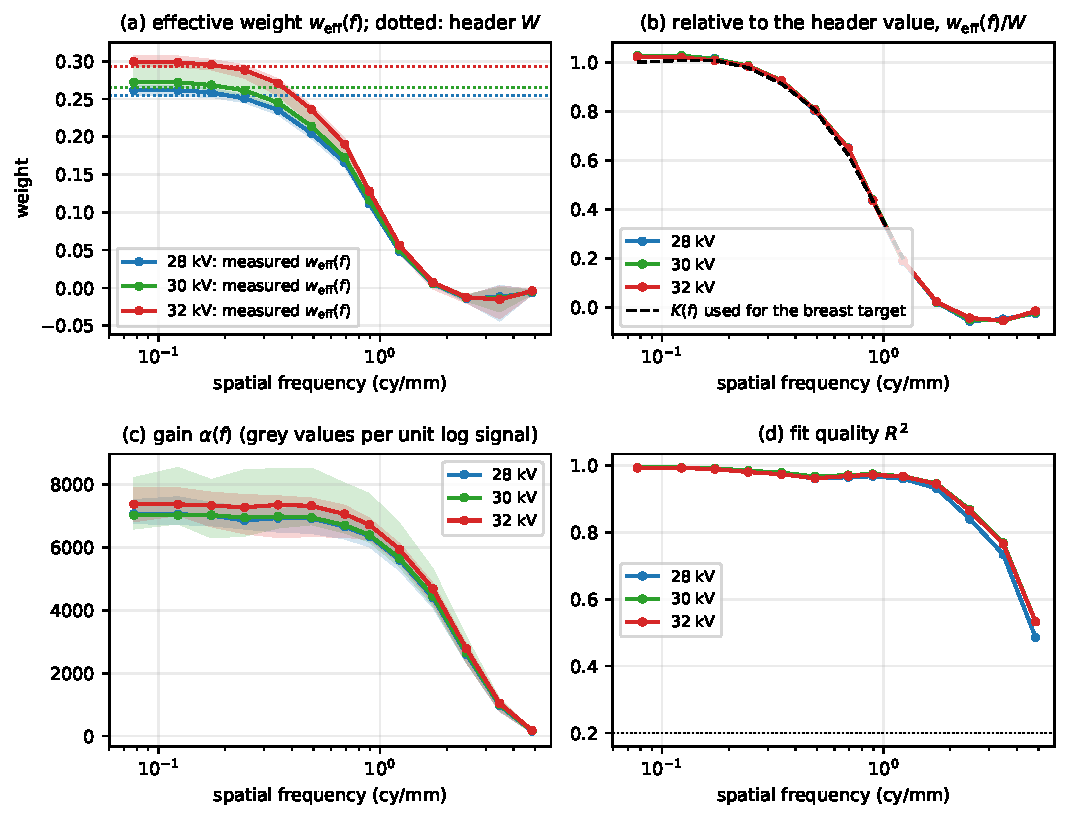
\includegraphics[width=\textwidth]{siemens_weighting.pdf}
\caption{Siemens' recombination measured from its own images (Eq.~\ref{eq:alphabeta}): median and range over the
exposures at each tube voltage. (b) includes the table $K(f)$ that was used for the breast target.}\label{fig:siemens}
\end{figure}

\begin{table}[H]\centering\small
\caption{Medians over the exposures per band: Siemens' effective weight $\weff$ at 28/30/32 kV, its gain and fit
quality at 28 kV, the cancelling weight $\ws$ of the L2 background, and the coherence at 28 kV.}\label{tab:siemens}
\begin{tabular}{r|rrr|rr|rrr|r}
\toprule
centre & \multicolumn{3}{c|}{$\weff$} & $\alpha$ & $R^2$ & \multicolumn{3}{c|}{$\ws$} & $\gamma^2$ \\
(cy/mm) & 28 & 30 & 32 & 28 & 28 & 28 & 30 & 32 & 28 \\
\midrule
0.077 & 0.262 & 0.272 & 0.300 & 7070 & 0.993 & 0.360 & 0.376 & 0.399 & 0.997 \\
0.122 & 0.262 & 0.272 & 0.299 & 7060 & 0.993 & 0.360 & 0.376 & 0.398 & 0.997 \\
0.173 & 0.259 & 0.268 & 0.295 & 7016 & 0.990 & 0.358 & 0.375 & 0.397 & 0.996 \\
0.245 & 0.251 & 0.261 & 0.288 & 6860 & 0.982 & 0.357 & 0.373 & 0.397 & 0.995 \\
0.346 & 0.235 & 0.245 & 0.271 & 6938 & 0.974 & 0.354 & 0.370 & 0.394 & 0.990 \\
0.490 & 0.205 & 0.214 & 0.236 & 6928 & 0.961 & 0.351 & 0.367 & 0.392 & 0.978 \\
0.693 & 0.166 & 0.172 & 0.190 & 6662 & 0.965 & 0.351 & 0.367 & 0.391 & 0.953 \\
0.894 & 0.111 & 0.116 & 0.128 & 6362 & 0.968 & 0.344 & 0.359 & 0.381 & 0.815 \\
1.225 & 0.048 & 0.051 & 0.056 & 5604 & 0.960 & 0.333 & 0.345 & 0.362 & 0.645 \\
1.732 & 0.006 & 0.006 & 0.007 & 4402 & 0.932 & 0.278 & 0.281 & 0.284 & 0.266 \\
2.449 & $-$0.014 & $-$0.013 & $-$0.012 & 2604 & 0.840 & 0.163 & 0.155 & 0.149 & 0.050 \\
3.464 & $-$0.012 & $-$0.014 & $-$0.016 & 972  & 0.734 & 0.066 & 0.073 & 0.062 & 0.007 \\
4.850 & $-$0.006 & $-$0.005 & $-$0.004 & 163  & 0.486 & 0.018 & 0.017 & 0.014 & 0.000 \\
\bottomrule
\end{tabular}
\end{table}

\subsection{What the linear model does not contain}\label{sec:nonlinear}
\begin{itemize}
\item \textbf{Large scales.} Siemens' image is flat at very low frequency. Below the first band the gain is taken to
fall as $f^2/(f^2+f_0^2)$ with $f_0=\SI{0.05}{cy/mm}$ (a fit from an earlier phantom pair)\As. In the method this only
decides how the correction is continued below 0.077\cymm.
\item \textbf{Edges.} In the outer $\approx$15 mm of the object Siemens applies a processing that is not a linear
function of the two log images (Section~\ref{sec:check}). Manufacturers describe a correction for the falling
thickness at the breast border \cite{korporaal2018,puong2007}.
\item \textbf{Mask and range.} Outside the object $R=0$; the values are limited to 0--4095.
\end{itemize}
The method does not need to reproduce any of these, because it keeps Siemens' image and only adds a correction
(Section~\ref{sec:idea}).

\subsection{Consequence for the L2 phantom}
The cancelling weight of the L2 background is $\ws=0.354$--0.366 at 28 kV, 0.369--0.382 at 30 kV and 0.392--0.404 at
32 kV\M. Siemens' weight is lower. By Eq.~\eqref{eq:rho} Siemens leaves the share
\begin{equation}
\rho_\mathrm{Siemens} = 1-\frac{\weff}{\ws}
\end{equation}
of the sphere contrast in the image: 26--28 \% at 28 kV, 22--29 \% at 30 kV and 24--26 \% at 32 kV
(medians 27.1 / 27.6 / 24.9 \%)\M. In breast tissue the same weight leaves much less: for the nine breast views the
cancelling weight at coarse scales is 0.245--0.276 against $W=0.244$--0.252, i.e.\ $1-W/\ws$ between $-0.03$ and
$+0.09$\M. The phantom background is therefore far stronger in Siemens' image than breast structure is.

Phantoms of spheres of several sizes in a liquid are an established way to give a physical phantom a breast-like,
power-law texture; the sphere sizes set the frequency range and the exponent \cite{gang2010,cockmartin2013,cockmartin2017}.
In CEM such texture is not removed by the system's own weighting, and residual texture influences iodine
measurements \cite{cockmartin2023,ding2017}; the amount of residual depends on the subtraction scheme
\cite{contillo2016}. In mammography phantoms, a textured background lowers detection scores compared with a uniform
one \cite{ikejimba2016}.

% =====================================================================================================================
\section{The breast target: how much structure Siemens' recombination leaves in real breasts}\label{sec:breast}

Breast structure acts as anatomical noise with a power-law spectrum, and it can limit detection more than quantum
noise does \cite{burgess2001,heine2002,bochud1999,richard2005}. In CEM the recombined image keeps a residual of it,
with a flatter spectrum than the LE and HE images \cite{hill2013b}. The tuned recombination needs a number for ``as
much background as in a breast''. It was measured once and is
stored in the script as the table \code{BREAST} (columns $T$ and $P_D$ of Table~\ref{tab:bands}).

\subsection{Data}
Nine views (CC and MLO) of two patients, acquired on another unit of the same system type: LE 27--28 kV W/Rh, HE
49 kV W/Ti, compressed thickness 34--47 mm, header weight $W=0.244$--0.252, pixel pitch 0.085 mm\Hd. The use of the
images was approved; only numbers were written.

\subsection{Preparation of each view}
\begin{enumerate}
\item \emph{Breast outline.} Pixels with HE value below 0.75 times the open-field level (the 99.5th percentile of
the HE image) are taken as breast; morphological opening (3 iterations), largest connected region, holes filled.
The image is mirrored if needed so that the chest wall is at column 0.
\item \emph{Distance to the skin line.} Euclidean distance of every breast pixel to the outline. Image borders that
the breast touches (chest wall; axilla in MLO views) are not counted as outline.
\item \emph{Log signals} by Eq.~\eqref{eq:log}.
\end{enumerate}

\subsection{Registration of the HE image onto the LE image}\label{sec:registration}
A patient moves between the two exposures; the phantom does not \cite{allec2012,sistermanns2021}. A shift between
$\LH$ and $\LL$ lowers their
coherence and would be counted as residual structure. Therefore $\LH$ is warped onto $\LL$ before the spectra are
taken:
\begin{enumerate}
\item Both log images are band-pass filtered: Gaussian of $\sigma=1.5$ pixels minus Gaussian of $\sigma=20$ pixels.
\item In windows of 256 pixels on a grid of 128 pixels that lie completely inside the breast, the local shift is
measured by phase correlation \cite{foroosh2002,zitova2003}: Hann window, normalised cross-power spectrum
$F_L\overline{F_H}/|F_L\overline{F_H}|$, inverse transform, position of the peak refined to sub-pixel accuracy by a
parabola through the peak and its two neighbours in each direction.
\item Shifts larger than 20 pixels are discarded. The remaining grid of shifts is median filtered ($3\times3$), empty
grid points are filled with the nearest value, and the grid is smoothed with a Gaussian of one grid step.
\item The shift field is interpolated bilinearly to every pixel and $\LH$ is resampled with cubic interpolation.
\end{enumerate}
The median shift per view was 0.15--0.66 mm (1.7--7.8 pixels; 56--114 windows per view)\M. After registration the two
log images explain Siemens' recombined image much better ($R^2$ at 0.06--0.15\cymm: 0.69--0.95 instead of 0.22--0.79),
and the frequency dependence $\weff(f)/W$ measured in the breasts equals that of the phantom (0.98--1.03, 0.75--0.82
and 0.37--0.52 at 0.1, 0.5 and 0.9\cymm)\M. This is the evidence that the same recombination, with the same LE
filter, is applied to breasts and to the phantom.

\subsection{Spectra}
ROIs as in Section~\ref{sec:spectra}, lying completely in the region that is at least 300 pixels (25.5 mm) inside the
skin line and more than 150 pixels (12.75 mm) away from the chest-wall image border: 68--203 ROIs per view. From them
$S_{LL}$, $S_{HH}$, $S_{HL}$ per band (Eq.~\ref{eq:psd}), with the registered $\LH$.

\subsection{Residual under Siemens' weighting}
The power of the weighted difference that Siemens forms is, for view $v$ and band $b$,
\begin{equation}
P_{D,v}(b) = S_{HH} - 2\,W_vK(b)\,S_{HL} + \big(W_vK(b)\big)^2 S_{LL},
\label{eq:PDbreast}
\end{equation}
with the header weight $W_v$ of that view and Siemens' LE filter $K(b)$ (Table~\ref{tab:bands}). The table $K$ is
the empirical filter fitted earlier on a phantom pair of an older unit of the same type (28 kV); it is 1 below
0.1\cymm\ by construction. Figure~\ref{fig:siemens}b shows that it agrees with $\weff/W$ measured on the 112 new
exposures.

\subsection{Quantum noise}\label{sec:noise}
$P_D$ contains quantum noise, which is not structure. Splitting an image power spectrum into quantum and
anatomical parts follows \cite{hill2013a}; quantum noise left in biases the power-law description of anatomical
noise \cite{mainprize2012}. It is removed with two assumptions\As:
\begin{enumerate}
\item In the highest band (4--5.88\cymm) the log images contain noise only.
\item The noise spectrum has the shape of white noise passed through the detector blur and sampled, with aliasing
\cite{dobbins1995,albert2000,cunningham2000}; direct-conversion selenium detectors are undersampled and their noise is
aliased \cite{zhao1997,zhao2003}. Along one axis
\begin{equation}
s(u)=\sum_{k=-2}^{2}\mathrm{MTF}\!\big(|u+k/p|\big)^2,
\end{equation}
and in two dimensions, averaged over the angle $\theta$ and over the band,
\begin{equation}
g(b)=\frac{\big\langle s(f\cos\theta)\,s(f\sin\theta)\big\rangle_{\theta,\,f\in b}}{\big\langle s(f\cos\theta)\,s(f\sin\theta)\big\rangle_{\theta,\,f\in B}},
\qquad B=\text{last band}.
\label{eq:g}
\end{equation}
\end{enumerate}
The presampling MTF is the published one of this detector type, 1.00 / 0.91 / 0.86 / 0.78 / 0.67 / 0.55 / 0.44 at
0--6\cymm\ \cite{nhsbsp}, continued as 0.34 / 0.25 / 0.18 / 0.13 / 0.09 / 0.06 / 0.03 / 0 at 7--14\cymm\As\ and
interpolated linearly. The average uses 64 angles between 0 and $\pi/2$ and 9 frequencies per band. The resulting
$g$ falls from 2.68 in the lowest band to 1 in the highest (Table~\ref{tab:bands}, Fig.~\ref{fig:breast}c).

The noise power in $D$ is then $N_v(b)=\big[S^\mathrm{raw}_{HH}(B) + (W_vK(b))^2S_{LL}(B)\big]\,g(b)$. The HE noise is
taken from the \emph{unregistered} HE image, because the resampling of the registration smooths the noise.

\subsection{Target}
The structured residual of view $v$ is $T_v(b)=\max\{P_{D,v}(b)-N_v(b),\,0\}$ and the target is the median over the
nine views,
\begin{equation}
T(b)=\operatorname*{median}_{v}\,T_v(b).
\label{eq:T}
\end{equation}
It is about \num{1e-5} mm$^2$ at 0.06--0.3\cymm, falls to \num{4e-7} mm$^2$ at 0.9\cymm\ and is zero from 1\cymm:
above 1\cymm\ Siemens' breast images contain no measurable structure, only noise (Fig.~\ref{fig:breast}). The views
differ by a factor of about five at the coarse scales (range in Table~\ref{tab:bands}). Recomputing the table from
the stored per-view spectra reproduces the numbers in the script (largest difference \num{4e-9} mm$^2$)\M.

\begin{figure}[H]\centering
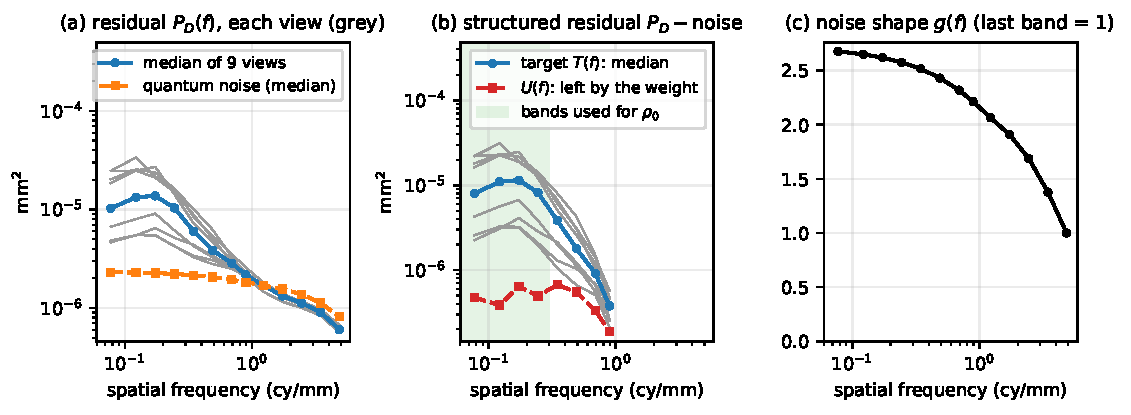
\includegraphics[width=\textwidth]{breast_target.pdf}
\caption{The breast target. (a) Total residual under Siemens' weighting in each of the nine views (grey), their
median, and the median noise estimate. (b) Structured residual of each view and the target $T$; the shaded bands are
the ones used to set the tuned weight. Dashed: the median over the views of $U$ (Eq.~\ref{eq:U}), the tissue
structure left by Siemens' weight. (c) The noise shape $g$ of Eq.~\eqref{eq:g}.}\label{fig:breast}
\end{figure}

\subsection{What the target consists of}\label{sec:origin}
The target is an amount of structure. Where that structure comes from can be read from Eq.~\eqref{eq:PDsplit}. With
the cancelling weight of the view's own tissue, $\ws_v(b)=S_{HL}/S_{LL}$ (registered spectra), the residual of
Eq.~\eqref{eq:PDbreast} is
\begin{equation}
P_{D,v}(b)=\underbrace{S_{HH}\,(1-\gamma^2)}_{\text{what LE does not predict, with the noise}}
\;+\;\underbrace{S_{LL}\,\big(W_vK(b)-\ws_v(b)\big)^2}_{U_v(b):\ \text{tissue structure left by the weight}} .
\label{eq:U}
\end{equation}
$U_v$ is glandular and adipose structure that both images share and that is not fully cancelled, because Siemens'
weight $W_vK$ is not exactly $\ws_v$. It is the only part that another weight could remove. The rest of the target,
$T_v-U_v$, is structure in the HE image that the LE image does not predict.

\begin{itemize}
\item Summed over the four bands 0.06--0.3\cymm, $U_v$ is 1.0--32.8 \% of $T_v$ in the nine views (median
14.1 \%); the median of $U$ over the views is 4--6 \% of the target $T$ in each of these bands\M. At these scales
Siemens' weight is close to the cancelling weight of the tissue ($\ws_v=0.245$--0.276 against
$W_v=0.244$--0.252).
\item Between 0.3 and 1\cymm\ the share is larger: the median of $U$ is 17, 31, 37 and 50 \% of the target in the
four bands\M, because $K$ falls there and less of the LE image is subtracted (Fig.~\ref{fig:breast}b).
\item The cause of the larger part, $T_v-U_v$, could not be determined from these data. Candidates are iodine in tissue
and vessels (the images are contrast-enhanced), tissue whose ratio of HE to LE contrast differs from that of the
main glandular--adipose structure, and registration error that remains\As. They were not separated. Background
parenchymal enhancement is visible in CEM recombined images \cite{sogani2017}, and iodine uptake in normal tissue
is named as one cause of incomplete cancellation \cite{hill2013b}.
\end{itemize}

For the phantom this means: the tuned image is matched to the breasts in the \emph{amount} of structured residual at
coarse scales, not in its origin. In the breasts most of that residual is not left-over background. The phantom has
less such content away from the discs: its own non-noise residual $E$ (Eq.~\ref{eq:E}) is below the target, 27 \% of
it in the worked example of Section~\ref{sec:design}. The script fills the difference with sphere structure that is
left in on purpose, 73 \% of the target power in that example\M.

% =====================================================================================================================
\section{The tuned recombination of the L2 images}\label{sec:tuned}

\subsection{Idea}\label{sec:idea}
By Eq.~\eqref{eq:model} Siemens' image is $\alpha[\LH-\weff\LL]+\text{rest}$. The wanted image is the same with
another weight, $\alpha[\LH-\wt\LL]+\text{rest}$. The two differ by $\alpha(\wt-\weff)\LL$, a filtered LE image
(combining images with frequency-dependent filters is the principle of measurement-dependent filtering
\cite{macovski1983,cao1988}).
Therefore
\begin{equation}
\boxed{\;R_\mathrm{tuned} = R - \mathcal F^{-1}\!\Big\{c(f)\,\mathcal F\{\LL\}\Big\},\qquad
c(f)=\alpha(f)\,\big[\wt(f)-\weff(f)\big]=\alpha(f)\,\wt(f)+\beta(f)\;}
\label{eq:tuned}
\end{equation}
Only the weight on the background changes. Everything else in Siemens' image -- its edge processing, the container
wall, the mask, the grey scale, the noise filtering, the iodine signal of $\LH$ -- stays exactly as Siemens made
it, because it is contained in $R$ and not touched. All quantities in Eq.~\eqref{eq:tuned} are measured from the
image that is processed; nothing is averaged over images.

\subsection{Step 1: object and interior}\label{sec:step1}
\begin{itemize}
\item \emph{Footprint.} HE value below 0.6 times the open-field level (99.5th percentile of the HE image), opening
with 3 iterations, largest connected region, holes filled. Example exposure: 268 cm$^2$.
\item \emph{Interior.} Pixels more than 25.5 mm inside the footprint outline (Euclidean distance transform) with
$0<R<4095$. Example: 120 cm$^2$.
\item \emph{ROIs.} All positions of the half-overlapping grid whose $128\times128$ pixels lie completely in the
interior: 293--325 per image\M\ (example: 320). The script stops if fewer than 30 are found.
\end{itemize}

\subsection{Step 2: regions that are left out automatically}\label{sec:select}
ROIs that contain an iodine disc, a bubble or the marker hold content that the LE image does not predict. They would
bias the weights and are removed without any template of the phantom:
\begin{enumerate}
\item With the current set of ROIs compute $\ws(b)$ by Eq.~\eqref{eq:wstar}.
\item For every ROI compute the residual power at that weight, $S_{HH}-2\ws S_{HL}+\ws{}^2S_{LL}$, summed over all DFT
samples between 0.1 and 1.0\cymm, and take its logarithm $\ell_j$.
\item Keep the ROIs with $\ell_j<\operatorname{median}(\ell)+3.5\cdot1.4826\cdot\operatorname{MAD}(\ell)$ (median and MAD
over the kept ones). Only the upper tail is cut. $1.4826\cdot\mathrm{MAD}$ is the robust estimate of the
standard deviation \cite{rousseeuw1993,leys2013}, and 3.5 is the limit recommended for the modified z-score
\cite{iglewicz1993}.
\item Repeat from 1 until the set no longer changes (at most 8 times).
\end{enumerate}
Typically 15--43 of the ROIs are left out and 261--303 are used\M\ (Fig.~\ref{fig:regions}; example: 27 left out, 293
used). The ROIs left out sit on the disc rows.

\begin{figure}[H]\centering
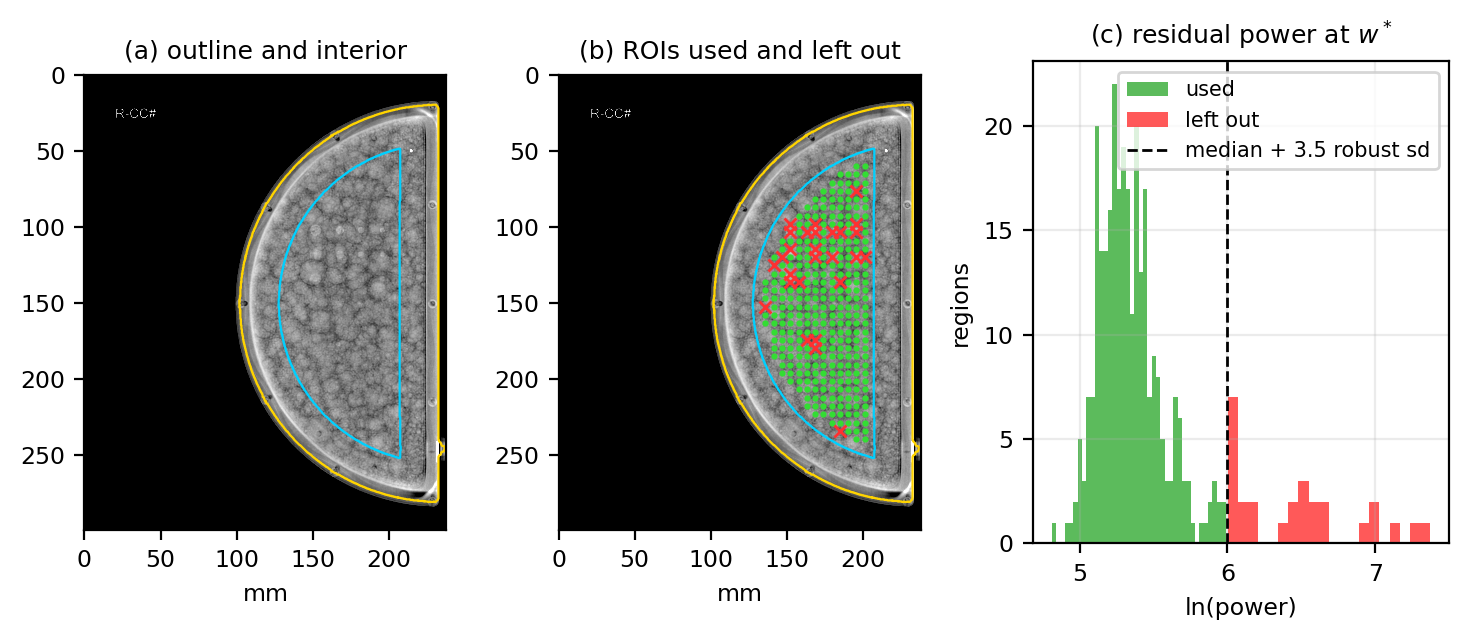
\includegraphics[width=\textwidth]{regions.png}
\caption{Example exposure (28 kV, normal level). (a) Siemens' recombined image with the footprint outline (yellow)
and the interior, 25.5 mm inside it (cyan). (b) Centres of the ROIs that are used and of those left out.
(c) The quantity on which the selection is made.}\label{fig:regions}
\end{figure}

\subsection{Step 3: measurements from the kept regions}
From the kept ROIs, per band: the six spectra of Section~\ref{sec:spectra}; the cancelling weight $\ws$
(Eq.~\ref{eq:wstar}), the coherence $\gamma^2$ and the cancellable power $C$ (Eq.~\ref{eq:C}); Siemens' gain $\alpha$,
$\beta$, $R^2$ and effective weight $\weff$ (Eq.~\ref{eq:alphabeta}). In addition the phantom's own
\emph{non-noise residual at full cancellation},
\begin{equation}
E(b)=\max\Big\{S_{HH}(b)\big(1-\gamma^2(b)\big)-\big[S_{HH}(B)+\ws(b)^2S_{LL}(B)\big]\,g(b),\;0\Big\},
\label{eq:E}
\end{equation}
i.e.\ what remains at $w=\ws$ after the quantum noise (estimated as in Section~\ref{sec:noise}, from the last band
$B$ of the same image) is taken off. $E$ is structure that even the best weight cannot remove; it already counts
towards the target.

The cancelling weight is constant up to about 0.7\cymm\ and then falls with the coherence
(Fig.~\ref{fig:wstar}, Table~\ref{tab:siemens}): where the two images no longer share structure, $S_{HL}/S_{LL}$ tends
to zero, so no LE noise is subtracted there. No separate LE filter is needed for that.

\begin{figure}[H]\centering
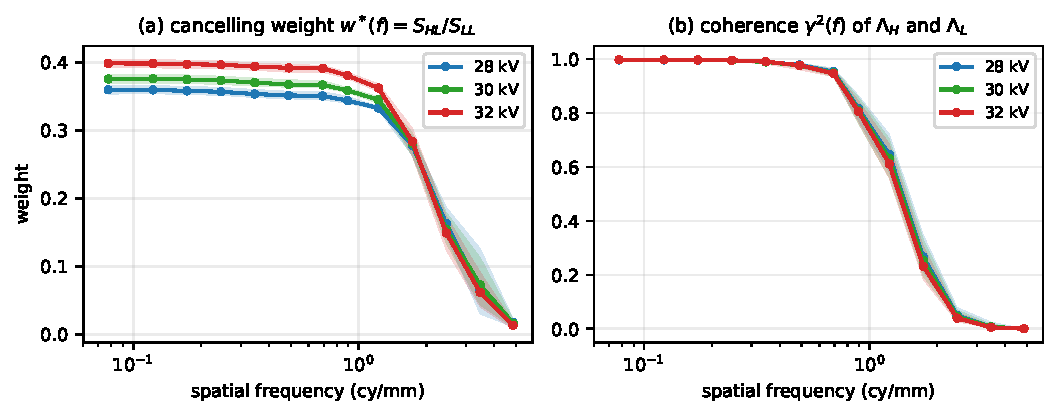
\includegraphics[width=0.95\textwidth]{wstar_coherence.pdf}
\caption{Cancelling weight and coherence of the L2 background: median and range over the exposures at each tube
voltage.}\label{fig:wstar}
\end{figure}

\subsection{Step 4: the tuned weight}\label{sec:design}
The tuned weight is $\wt(b)=\ws(b)\,[1-\rho(b)]$. By Eqs.~\eqref{eq:rho} and \eqref{eq:E} the structured residual it
leaves is $E+\rho^2C$. One share $\rho_0$ is chosen for the coarse scales so that this equals the breast target,
summed over the four bands below 0.3\cymm\ (0.06--0.30\cymm):
\begin{equation}
\rho_0(s)=s\,\sqrt{\frac{\max\Big\{\sum_{b:\,f_b<0.3}\big[T(b)-E(b)\big],\,0\Big\}}{\sum_{b:\,f_b<0.3}C(b)}}\,,
\qquad \rho_0\le0.6 .
\label{eq:rho0}
\end{equation}
$s$ is the \emph{strength}: $s=1$ leaves as much structure as Siemens leaves in the breasts, $s=0$ is full
cancellation, $s=0.5$ and $s=2$ half and double the share. (The script notes that $s=2$ is about the grey-level
texture of Siemens' breast images, because Siemens' gain was found 1.6--2 times higher for the breast images than
for the phantom; that is an earlier measurement and is not used in the calculation.) The share is then faded out
smoothly towards fine scales, where the breasts have no structure, with a raised-cosine taper as used for data
windows \cite{harris1978}:
\begin{equation}
\rho(f)=\rho_0\cdot\tfrac12\big[1+\cos(\pi u)\big],\qquad
u=\min\!\Big\{\max\!\Big\{\frac{\log_{10}f-\log_{10}0.3}{\log_{10}1.0-\log_{10}0.3},0\Big\},1\Big\},
\label{eq:fade}
\end{equation}
evaluated at the band centres: $\rho=\rho_0$ up to 0.3\cymm\ and $\rho=0$ from 1\cymm.

The two limits are a choice, read from the breast target and not fitted\As. $T$ is of one size in the four bands up
to 0.3\cymm\ (\num{8.0e-6}--\num{1.15e-5} mm$^2$), it is less than half of that in the next band (0.3--0.4\cymm:
\num{3.9e-6} mm$^2$), and no structure is measurable from 1\cymm\ (Section~\ref{sec:breast},
Fig.~\ref{fig:breast}b). The cosine shape of the fade on a logarithmic frequency axis is also a choice.

Remarks.
\begin{itemize}
\item A single share for all coarse bands scales the phantom's own structure down and keeps its character; the
spectrum of the remaining structure is that of the spheres, not that of a breast.
\item The four bands enter Eq.~\eqref{eq:rho0} with equal weight (plain sums of the band values).
\item \emph{Worked example} (28 kV, normal level, first exposure): $\sum C=\num{6.00e-3}$, $\sum T=\num{3.86e-5}$,
$\sum E=\num{1.06e-5}$ mm$^2$, hence $\rho_0=\sqrt{\num{2.80e-5}/\num{6.00e-3}}=0.068$: 6.8 \% of the sphere contrast is
left in, where Siemens leaves 27 \%. With $\ws=0.360$ the tuned weight at coarse scales is $0.360\cdot0.932=0.336$
(Siemens: 0.263).
\end{itemize}

\begin{figure}[H]\centering
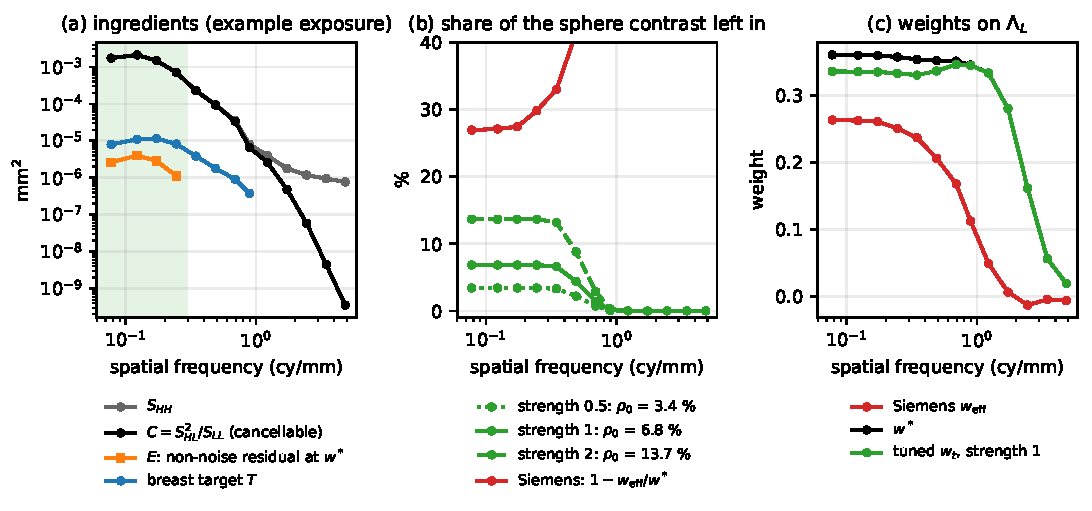
\includegraphics[width=\textwidth]{design.pdf}
\caption{Design of the tuned weight for the example exposure. (a) The quantities of Eq.~\eqref{eq:rho0}. (b) The
left-in share for three strengths and Siemens' share, which rises to 100 \% above 1.5\cymm\ (off the scale). (c) The
resulting weights.}\label{fig:design}
\end{figure}

\subsection{Step 5: applying the correction to the whole image}\label{sec:apply}
The band values of the correction filter are
\begin{equation}
c(b)=\begin{cases}\alpha(b)\,\wt(b)+\beta(b), & R^2(b)\ge0.2\\ 0, & \text{otherwise}\end{cases}
\end{equation}
(in the 112 exposures $R^2\ge0.2$ in every band, so no band was switched off\M). The filter is applied to the whole LE
log image as a radial filter in the Fourier domain:
\begin{enumerate}
\item \emph{Continuation outside the object.} The LE log image has a large step at the phantom edge. To keep this
step from spreading into the phantom through the filter, the image is replaced outside the footprint (dilated by
10 pixels) by a smooth continuation of the inside: with the mask $m$,
$\tilde\Lambda=\big(G_{60}*(m\LL)\big)/\big(G_{60}*m\big)$, $G_{60}$ a Gaussian of $\sigma=60$ pixels (5.1 mm); far outside,
the mean inside value.
\item \emph{Padding.} 256 pixels on every side by reflection, enlarged to the next fast FFT size. Continuation
and padding avoid the border artefacts of Fourier filtering \cite{moisan2011,liu2008}.
\item \emph{Filter.} For the radial frequency $f$ of every Fourier sample, $c$ is interpolated linearly in
$\log_{10}f$ between the band centres and held constant above the last centre. Below the first centre
$f_1=\SI{0.077}{cy/mm}$ it follows Siemens' large-scale roll-off,
\begin{equation}
c(f)=c(b_1)\,\frac{g_0(f)}{g_0(f_1)},\qquad g_0(f)=\frac{f^2}{f^2+f_0^2},\quad f_0=\SI{0.05}{cy/mm},
\label{eq:rolloff}
\end{equation}
so that $c(0)=0$: the mean level and the largest scales of Siemens' image are not changed.
\item \emph{Result.} Inverse transform, cut back to the image size, and
$R_\mathrm{tuned}=\operatorname{round}\big(R-\text{correction}\big)$, limited to 0--4095 and set to 0 where $R=0$
(Siemens' mask is kept).
\end{enumerate}
Figure~\ref{fig:filter} shows the filter. It is about 510--550 grey values per unit log signal at coarse scales and
rises to 1600--1800 in the band 1.0--1.5\cymm, because there Siemens subtracts little LE ($K$ is small) while the tuned
weight is still the full cancelling weight: this is where the fine sphere edges are removed. Above 2\cymm\ it falls
to zero, as the coherence and Siemens' gain fall.

\begin{figure}[H]\centering
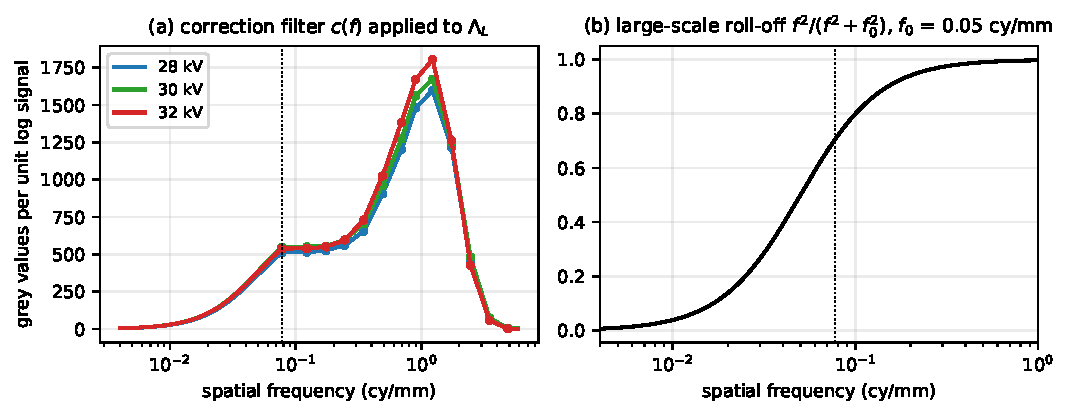
\includegraphics[width=0.95\textwidth]{filter.pdf}
\caption{(a) The correction filter of Eq.~\eqref{eq:tuned} for one normal-level exposure per tube voltage: band
values (dots) and the interpolated filter. (b) The roll-off of Eq.~\eqref{eq:rolloff} below the first band
centre (dotted line).}\label{fig:filter}
\end{figure}

\subsection{What is smoothed, and how shading is avoided}
\begin{itemize}
\item The image itself is not smoothed. $R$ is kept pixel by pixel; the correction is a filtered LE image whose
filter falls to zero at high frequency, so it adds no LE noise.
\item Smoothness enters in four places only: the averaging of the spectra over ROIs and bands; the interpolation
of the filter between band centres on a logarithmic frequency axis; the cosine fade of the share
(Eq.~\ref{eq:fade}); and the smooth continuation outside the object.
\item Shading (slow brightness changes) is not introduced, because $c(f)\to0$ for $f\to0$
(Eq.~\ref{eq:rolloff}) and because ROIs are detrended before the weights are measured, so slow trends do not
influence them.
\item Halos at the wall are avoided by the continuation and the padding of step~1 and~2. Siemens' own edge
processing stays, since $R$ is kept.
\end{itemize}

\subsection{Step 6: check on the result and output}
The regression of Section~\ref{sec:regression} is repeated on the tuned image in the same ROIs. The weight found in
the tuned image agrees with the designed one within 0.0014 (mean difference $+0.0006$) in all 112
exposures\M\ (Fig.~\ref{fig:summary}c). The tuned image is written as a copy of Siemens' DICOM file with new pixel
data, new instance and series UIDs, a series description and an image comment that mark it as research output.

For every image the script also writes the curves (weights, share, residual spectra; PNG and CSV) and a comparison
picture, and collects all numbers in \code{L2\_tuned\_recombination\_numbers.xlsx}.

% =====================================================================================================================
\section{Results on the 112 exposures (strength 1)}\label{sec:results}

\begin{table}[H]\centering\small
\caption{Medians per group at coarse scales (0.06--0.15\cymm): Siemens' effective weight, the cancelling weight, the
tuned weight, and the share of the sphere contrast left in by Siemens and by the tuned recombination.}\label{tab:results}
\begin{tabular}{llrrrrrr}
\toprule
kV & level & $\weff$ & $\ws$ & $\wt$ & Siemens share (\%) & tuned share (\%) & ROIs used / left out \\
\midrule
28 & low    & 0.264 & 0.364 & 0.338 & 27.2 & 7.2 & 294 / 23 \\
28 & normal & 0.261 & 0.360 & 0.336 & 27.5 & 6.6 & 286 / 28 \\
28 & high   & 0.259 & 0.355 & 0.332 & 27.0 & 6.5 & 278 / 29 \\
30 & low    & 0.276 & 0.380 & 0.355 & 27.5 & 6.6 & 280 / 29 \\
30 & normal & 0.273 & 0.376 & 0.352 & 27.5 & 6.3 & 277 / 29 \\
30 & high   & 0.268 & 0.370 & 0.346 & 27.6 & 6.6 & 274 / 32 \\
32 & low    & 0.303 & 0.404 & 0.377 & 24.9 & 6.7 & 278 / 25 \\
32 & normal & 0.299 & 0.398 & 0.374 & 25.0 & 6.2 & 279 / 27 \\
32 & high   & 0.297 & 0.395 & 0.371 & 24.6 & 6.0 & 277 / 26 \\
\bottomrule
\end{tabular}
\end{table}

\begin{itemize}
\item The tuned share is 5.4--7.8 \% in all exposures but one (3.5 \% in one 32 kV exposure), against 22--29 \% for
Siemens\M. It is 0.1--0.7 percentage points higher at the low exposure level than at the other two; the cause was
not examined.
\item The residual spectrum of the tuned images lies inside the range of the nine breast views at all frequencies
(Fig.~\ref{fig:spectra}). At 0.2--0.3\cymm\ the residual power is \num{6.3e-5}--\num{7.1e-5} mm$^2$ under Siemens'
weighting, \num{7.0e-6} mm$^2$ tuned, and \num{1.0e-5} mm$^2$ (range \num{4.2e-6}--\num{1.6e-5}) in the
breasts\M. (The match of Eq.~\eqref{eq:rho0} is on the structured part summed over 0.06--0.3\cymm, not on the total
power of one band.)
\item The cancelling weight differs between exposure levels by 0.009 (28 kV: 0.355 high, 0.364 low). It is measured
per image, so this does not affect the result; its cause was not examined here.
\end{itemize}

\begin{figure}[H]\centering
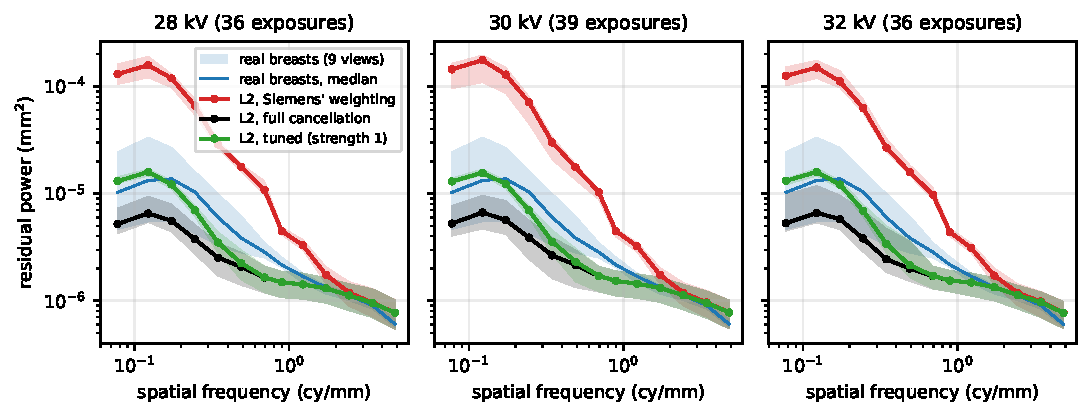
\includegraphics[width=\textwidth]{residual_spectra.pdf}
\caption{Power of the residual $\LH-w(f)\LL$ in the interior of the L2 phantom for Siemens' weighting, full
cancellation and the tuned weight (median and range over the exposures), against the nine breast views under
Siemens' weighting.}\label{fig:spectra}
\end{figure}

\begin{figure}[H]\centering
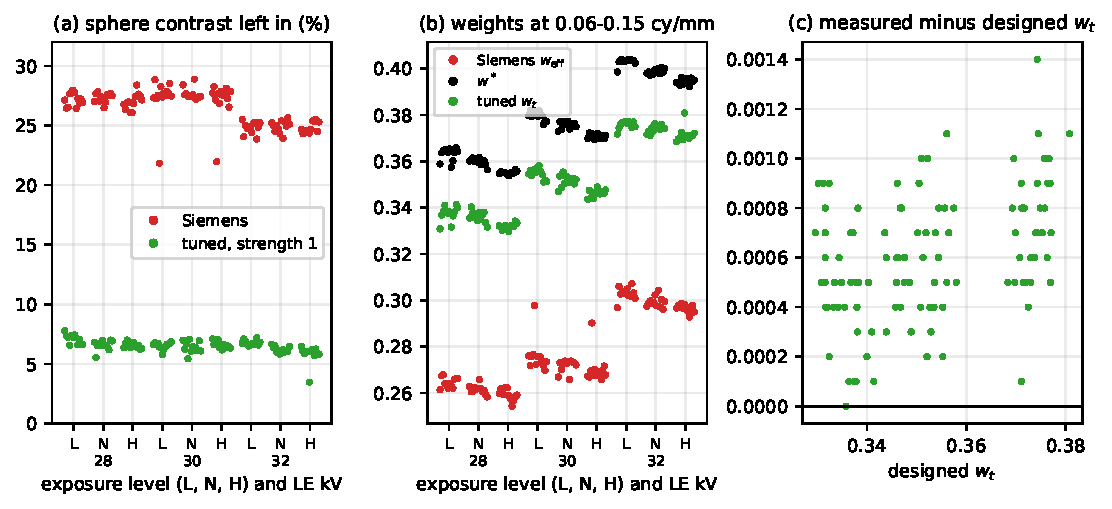
\includegraphics[width=\textwidth]{summary.pdf}
\caption{All 112 exposures, one dot each. (a) Share of the sphere contrast left in. (b) Weights at coarse scales.
(c) Weight measured in the tuned image minus the designed weight.}\label{fig:summary}
\end{figure}

\begin{figure}[H]\centering
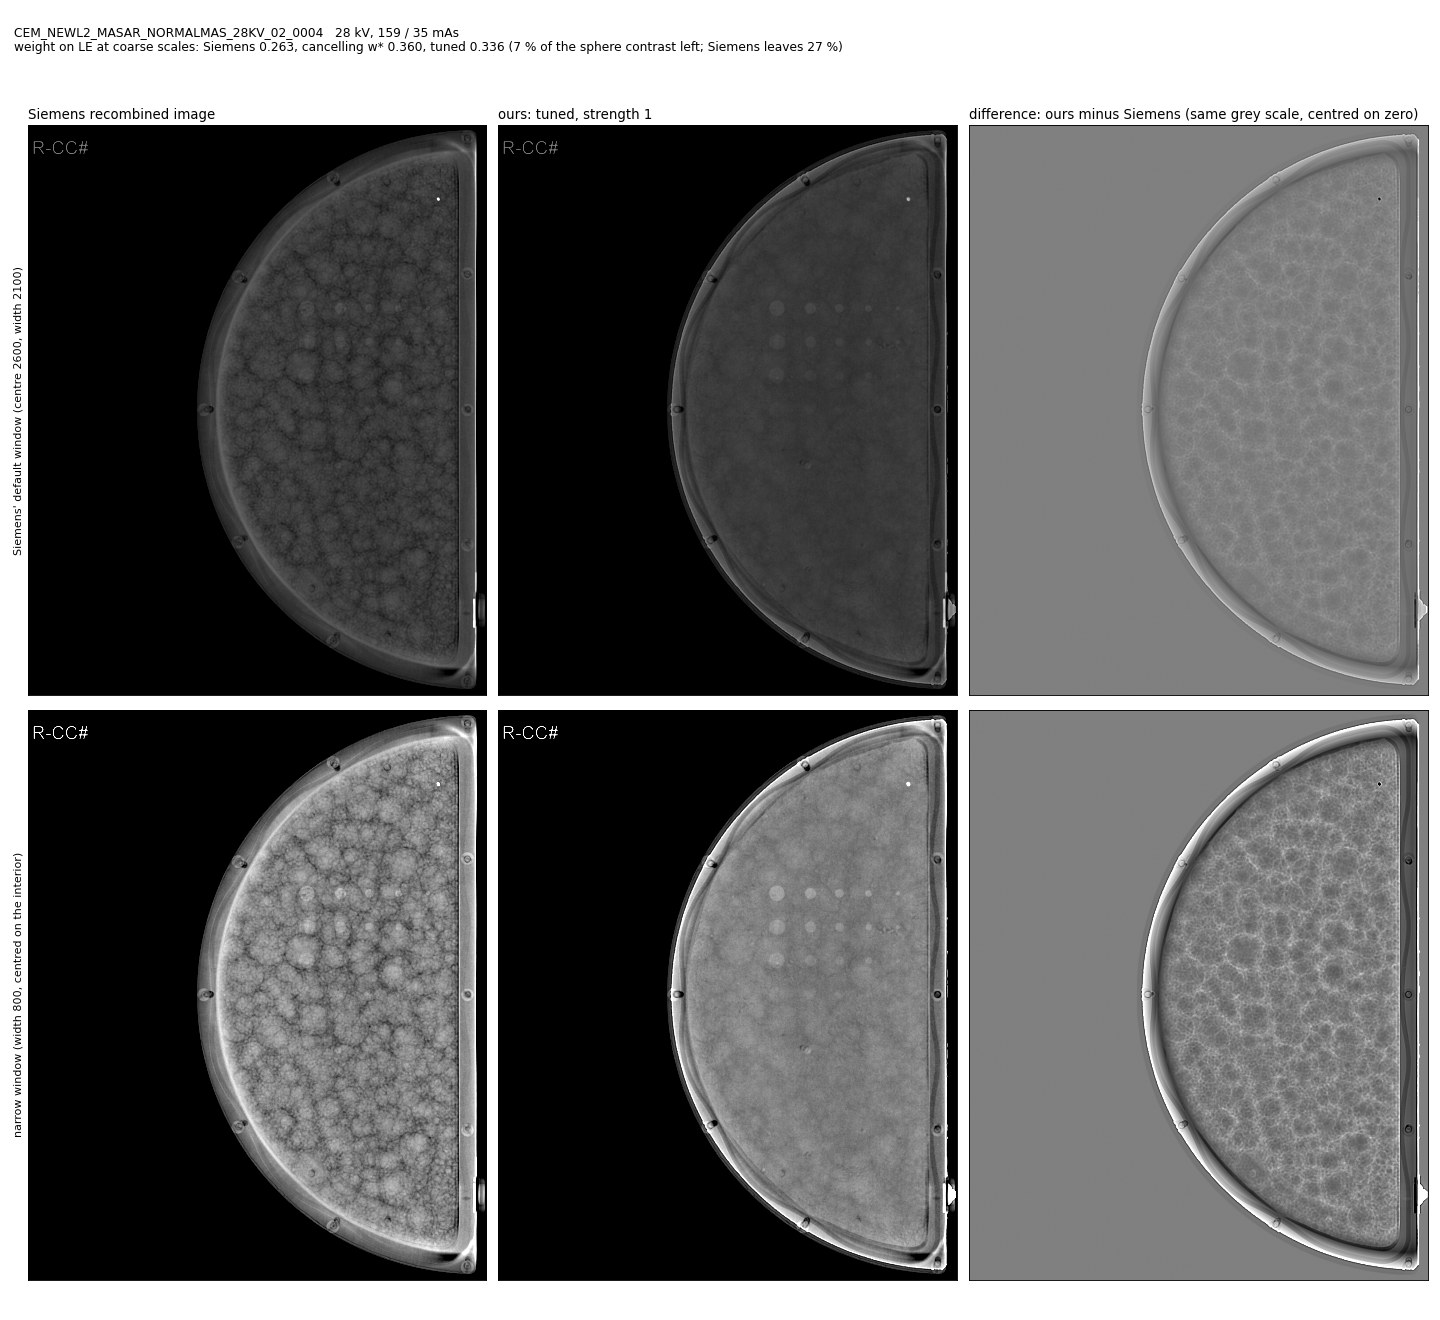
\includegraphics[width=0.93\textwidth]{comparison_tuned.jpg}
\caption{The comparison picture that the script writes for every exposure (here the example exposure): Siemens'
recombined image, the tuned image, and their difference (tuned minus Siemens). Top row: Siemens' default display
window (centre 2600, width 2100). Bottom row: a narrow window of width 800 centred on the interior median; the
difference is shown with the same window widths, centred on zero.}\label{fig:comparison}
\end{figure}

% =====================================================================================================================
\section{Check of the method: recombining the raw images at Siemens' own weighting}\label{sec:check}

If Eq.~\eqref{eq:model} and its measurement are right, the raw LE and HE images recombined with the measured
$\alpha$ and $\weff$ must reproduce Siemens' image. With the option \code{-{}-siemens-weighting} the script computes
\begin{equation}
R_\mathrm{ours}=\text{offset}+\mathcal F^{-1}\Big\{\alpha(f)\,\mathcal F\{\LH\}+\beta(f)\,\mathcal F\{\LL\}\Big\},
\label{eq:check}
\end{equation}
both filters applied as in Section~\ref{sec:apply} (bands with $R^2<0.2$ set to zero), the offset being the median of
$R-\mathcal F^{-1}\{\ldots\}$ more than 15 mm inside the outline. Three numbers are reported per image: the pixel-wise
correlation and rms difference with Siemens' image more than 15 mm inside the outline; the correlation in the outer
15 mm; and the share of Siemens' image that is reproduced, $100\,(1-P_\mathrm{diff}/P_R)$, with the powers of the
difference image and of $R$ summed over the bands up to 1\cymm\ in the kept ROIs.

\begin{table}[H]\centering\small
\caption{Check at Siemens' weighting: median (lowest--highest) over the exposures\M.}\label{tab:check}
\begin{tabular}{rrcccc}
\toprule
 & & interior & rms difference & reproduced (\%), & outer 15 mm \\
kV & $n$ & correlation & / image SD & 0.06--1\cymm & correlation \\
\midrule
28 & 36 & 0.957 (0.943--0.967) & 21.6 / 74.7 & 99.0 (98.0--99.4) & 0.62 (0.58--0.64) \\
30 & 39 & 0.963 (0.950--0.974) & 20.4 / 75.2 & 99.2 (98.3--99.6) & 0.62 (0.53--0.65) \\
32 & 36 & 0.954 (0.941--0.964) & 22.6 / 75.5 & 99.0 (97.4--99.5) & 0.61 (0.60--0.65) \\
\bottomrule
\end{tabular}
\end{table}

In the interior the linear model reproduces Siemens' image: 97--99.6 \% of its power up to 1\cymm, and the same
effective weight in both images (Fig.~\ref{fig:check}). Above 1\cymm\ the share reproduced falls, to 53--59 \% in the
highest band. In the regions used, the difference between the two images is about 10 grey values rms (from the
spectra), roughly half of it from the bands above 1\cymm\M. The pixel-wise figure of 20--23 grey values (image standard
deviation 75) is larger because it covers everything more than 15 mm inside the outline: scales below 0.06\cymm,
which detrending removes from the ROIs, the ring between 15 and 25.5 mm from the outline, and the disc regions. In
the outer 15 mm the agreement is poor (correlation 0.53--0.65): there Siemens
applies processing that is not in the model (Section~\ref{sec:nonlinear}). This is the reason why the tuned image is
built as ``Siemens' image plus a correction'' (Eq.~\ref{eq:tuned}) and not recombined from the raw images.

\begin{figure}[H]\centering
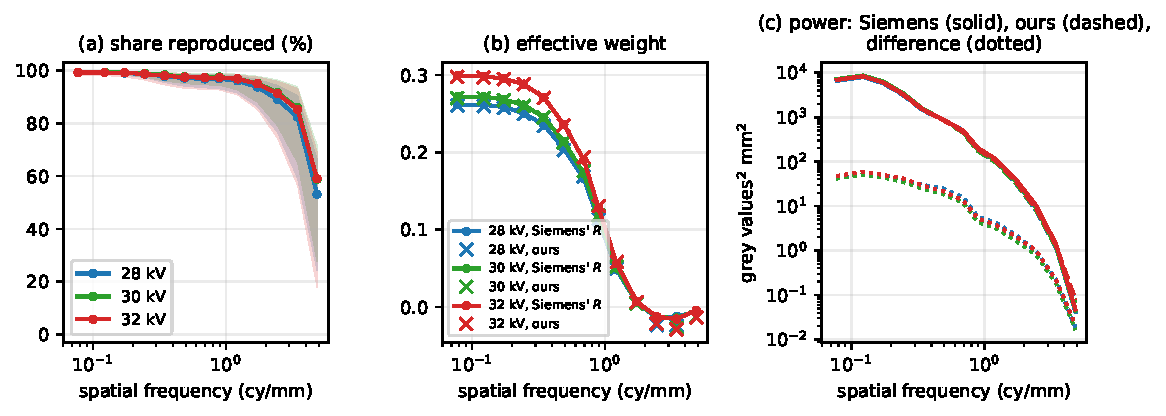
\includegraphics[width=\textwidth]{check.pdf}
\caption{Check at Siemens' weighting, medians (and range in a) over the exposures per tube voltage. (a) Share of
Siemens' image that ours reproduces per band. (b) Effective weight in Siemens' image (line) and in ours (crosses).
(c) Power spectra of Siemens' image, of ours and of their difference.}\label{fig:check}
\end{figure}

\begin{figure}[H]\centering
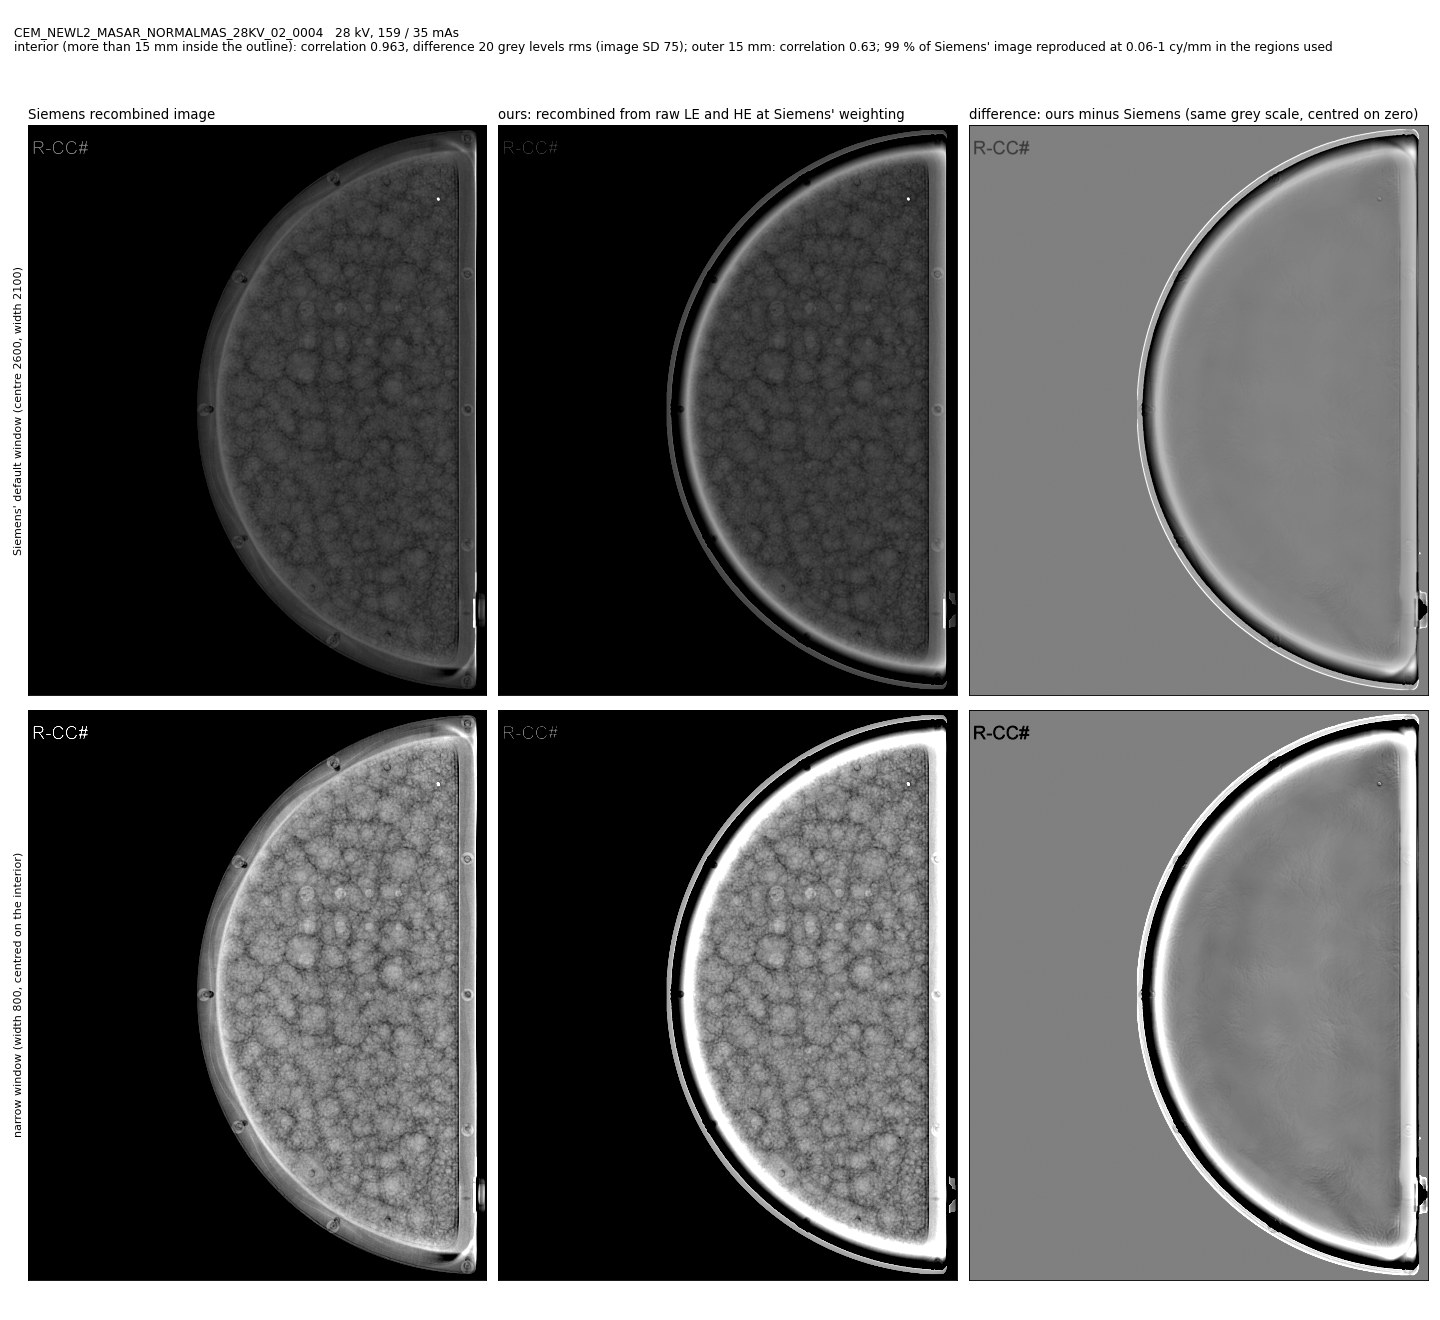
\includegraphics[width=0.93\textwidth]{comparison_check.jpg}
\caption{Check for the example exposure: Siemens' recombined image, our recombination of the raw LE and HE images
at Siemens' weighting (Eq.~\ref{eq:check}), and the difference. Windows as in Fig.~\ref{fig:comparison}.}\label{fig:checkimage}
\end{figure}

% =====================================================================================================================
\section{The same method on Hologic images}\label{sec:hologic}

The script \code{l2\_tuned\_recombination\_multisystem.py} applies the method of Sections~\ref{sec:tuned}--\ref{sec:check}
to images of the same L2 phantom from a Hologic Selenia Dimensions. Every step and every fixed number is the same;
only what depends on the system changes (Section~\ref{sec:hologicprofile}, Table~\ref{tab:profiles}). On a Siemens
exposure the multi-system script gives the same tuned image and the same check image, pixel for pixel, and the same
curves as \code{l2\_tuned\_recombination.py}\M.

\subsection{Data}
Fifteen CEM acquisitions of the L2 with the new plate (22 October 2026), CC view, each with a raw LE and a raw HE image
(FOR PROCESSING, 14 bit) and Hologic's recombined image DES (12 bit, logarithmic)\Hd. The automatic exposure control
(AutoFilter) chose 29 kV for 8 and 30 kV for 7 exposures. Compressed thickness 54--56 mm; compression force mostly
about 61 N (25--101 N)\Hd. The phantom background differs between exposures: the band-pass filtered LE images of seven
pairs of exposures correlate by 0.00--0.25\M, so the phantom was moved or shaken between them. Table~\ref{tab:acq}
compares the acquisition with the Siemens normal level. The doses are the manufacturers' own estimates in the headers
and were not recalculated. Test methods for CEM systems of several manufacturers, including textured backgrounds,
are compared in \cite{cockmartin2023}.

\begin{table}[H]\centering\small
\caption{Acquisition from the headers\Hd: median per group. Siemens at the normal exposure level (AEC dose level
149~\%); the low and high levels are in \code{system\_comparison.xlsx}.}\label{tab:acq}
\footnotesize\setlength{\tabcolsep}{3pt}
\begin{tabular}{lccccc}
\toprule
 & \multicolumn{2}{c}{Hologic Selenia Dimensions} & \multicolumn{3}{c}{Siemens MAMMOMAT Revelation} \\
 & 29 kV & 30 kV & 28 kV & 30 kV & 32 kV \\
\midrule
exposures & 8 & 7 & 12 & 12 & 12 \\
LE anode / filter & \multicolumn{2}{c}{W / Ag 0.05 mm} & \multicolumn{3}{c}{W / Rh 0.05 mm} \\
LE HVL (mm Al) & 0.569 & 0.586 & \multicolumn{3}{c}{not in the header} \\
HE & \multicolumn{2}{c}{49 kV, W / Cu 0.3 mm, HVL 3.24 mm Al} & \multicolumn{3}{c}{49 kV, W / Ti 1.0 mm} \\
mAs LE / HE & 97.5 / 77.8 & 97.0 / 86.3 & 161 / 34.9 & 122 / 35.0 & 92.3 / 34.8 \\
ratio mAs HE / LE & 0.80 & 0.89 & 0.22 & 0.28 & 0.38 \\
AGD LE + HE (mGy) & 1.40 + 0.69 & 1.54 + 0.75 & 1.62 + 0.56 & 1.49 + 0.56 & 1.34 + 0.56 \\
HE share of AGD & 33 \% & 33 \% & 26 \% & 27 \% & 30 \% \\
ESD LE / HE (mGy) & 4.81 / 0.75 & 5.25 / 0.83 & 6.11 / 0.65 & 5.44 / 0.65 & 4.72 / 0.65 \\
thickness / force & 54 mm / 61 N & 55 mm / 61 N & 54 mm / 50 N & 54 mm / 51 N & 54 mm / 53 N \\
\bottomrule
\end{tabular}
\end{table}

Both detectors are direct (a-Se), with 0.070 mm pixels on Hologic and 0.085 mm on Siemens. Source--detector distance
is 700 against 656 mm, and the magnification in the header 1.073 against 1.027. Both have a grid, 14-bit raw images
and a 12-bit recombined image\Hd. Hologic puts a much larger part of the exposure into the HE image.

\subsection{What the script changes for Hologic}\label{sec:hologicprofile}
\begin{itemize}
\item \emph{Finding the images.} The DES has the image type SUBTRACTION. It names only the irradiation event of
the HE image; the LE image is the one with the same acquisition time.
\item \emph{Bands and ROIs.} With 0.070 mm pixels a ROI has 156 pixels (10.9 mm, as on Siemens). The band edges are
the same up to 4\cymm; the last band, the noise reference, runs from 4\cymm\ to the Nyquist frequency of 7.14\cymm.
All other lengths (margin, continuation, padding, outline opening) are kept in mm.
\item \emph{Outline.} Same rule as in step 1 (Section~\ref{sec:step1}). Part of the HE open field is saturated (stored value
16383 at the image's upper edge), so saturated pixels are left out when the open-field level is taken. No Siemens
image has a saturated pixel, so nothing changes there.
\item \emph{Noise shape} $g$ (Eq.~\ref{eq:g}). No published MTF of this detector was available: the 2D evaluation
(NHSBSP report 1101) could not be obtained. $g$ was therefore measured once, in the open field of the 15
exposures. In ROIs lying completely in the open field, the power of $\LH-0.41\,\LL$ per band was taken relative to
the last band, and the median over the exposures is stored in the script (Fig.~\ref{fig:hologic}d). The single
exposures differ from it by at most 0.31. The open field also holds large-scale structure that is not quantum noise
(the peak at 0.15--0.2\cymm), so the lowest bands are an upper estimate\As. Using a flat $g=1$ or the Siemens shape instead changes the
left-in share by at most 0.4 percentage points (two exposures tested)\M.
\item \emph{Weight in the header.} Hologic writes none, so only the measured effective weight is reported. A private
tag of the DES holds 2 kB of binary data that could not be read. The software list names modules called
\code{CEDMSub} and \code{CEDMGetk}. This suggests that the weight is determined for each exposure, but it was not
verified\As.
\item \emph{Breast target.} The Siemens table is used unchanged (Section~\ref{sec:hologictarget}).
\item \emph{Comparison picture.} The top row uses Hologic's own default window (centre 2150, width 260). The second
row has a width of 380 grey values: Hologic's gain is about half of Siemens', so this is about the same width in log
signal as Siemens' 800.
\end{itemize}

\subsection{Hologic's recombination as it appears in its images}
The model of Eq.~\eqref{eq:model} describes the DES as well as it describes Siemens' image. In the regions used, $R^2$ is at least
0.98 up to 1\cymm, 0.94 at 1.0--1.5, 0.87 at 1.5--2 and 0.52 at 2--3\cymm. Above 3\cymm\ it is 0.11 or less, so
those bands are not corrected\M.
\begin{itemize}
\item \emph{Weight.} The effective weight is 0.313 (29 kV) and 0.310 (30 kV) at coarse scales and stays within 0.005
of that up to 2\cymm\M\ (Fig.~\ref{fig:hologic}a). Hologic weights the LE image at all scales alike, whereas Siemens
subtracts less and less LE above 0.2\cymm\ (its filter $K$).
\item \emph{Gain.} About 3390 grey values per unit log signal at coarse scales, 2990 at 0.6--0.8, 2050 at 1.0--1.5
and 320 at 2--3\cymm\M. Hologic smooths the whole recombined image at fine scales; Siemens smooths only the LE part.
\item \emph{Phantom.} The cancelling weight is 0.410 (29 kV) and 0.412 (30 kV). Hologic's weight leaves 23.6 and
24.7~\% of the sphere contrast, against 25--27.5~\% for Siemens (Fig.~\ref{fig:hologic}b).
\end{itemize}

\subsection{Breast target for Hologic}\label{sec:hologictarget}
There are no raw Hologic breast images, so the residual that Hologic's recombination leaves in breasts could not be
measured. The Siemens target $T$ is used unchanged, in log-signal units\As. It is a reasonable starting point but not
a measurement:
\begin{itemize}
\item Both systems set their weight to cancel breast tissue: Hologic's white papers state that parenchymal tissue
is subtracted \cite{alsheik2020,smith2014}, Siemens' that the anatomical background is neutralised
\cite{korporaal2018}. In the Siemens breasts most of the target is content that the LE image does not predict,
not tissue left by the weight (Section~\ref{sec:origin}).
\item The spectra differ (Table~\ref{tab:acq}). The iodine contrast per unit and the noise in log units may therefore
differ, and with them the residual that real breasts would show on Hologic. This was not quantified.
\item With this target the left-in share comes out at 6.3--6.9~\% on Hologic (Table~\ref{tab:hologic}), inside the
5.4--7.8~\% found on Siemens. The alternative, the same share as on Siemens (option \code{-{}-share}), would give
nearly the same images.
\end{itemize}

\subsection{Results}
\begin{table}[H]\centering\small
\caption{Hologic, strength 1, and the check at Hologic's own weighting: median (lowest--highest) over the
exposures\M. Weights at 0.06--0.15\cymm.}\label{tab:hologic}
\begin{tabular}{lcc}
\toprule
 & 29 kV ($n=8$) & 30 kV ($n=7$) \\
\midrule
Hologic's effective weight $\weff$ & 0.313 (0.312--0.315) & 0.310 (0.308--0.311) \\
cancelling weight $\ws$ & 0.410 (0.406--0.414) & 0.412 (0.410--0.416) \\
tuned weight $\wt$ & 0.383 (0.378--0.386) & 0.386 (0.383--0.387) \\
share left by Hologic & 23.6 \% (23.0--24.2) & 24.7 \% (24.4--25.8) \\
share left, tuned & 6.6 \% (6.4--6.9) & 6.5 \% (6.3--6.9) \\
ROIs used / left out & 275 / 35 & 279 / 36 \\
residual at 0.2--0.3\cymm, Hologic / tuned (mm$^2$) & \num{4.9e-5} / \num{5.5e-6} & \num{5.7e-5} / \num{5.4e-6} \\
\midrule
check: interior correlation & 0.928 (0.923--0.939) & 0.937 (0.919--0.941) \\
check: rms difference / image SD (grey values) & 11.7 / 30.4 & 11.0 / 30.5 \\
check: reproduced at 0.06--1\cymm & 99.9 \% & 99.9 \% \\
check: correlation in the outer 15 mm & 0.18 (0.12--0.31) & 0.17 (0.13--0.20) \\
\bottomrule
\end{tabular}
\end{table}

\begin{itemize}
\item The weight measured in the tuned image agrees with the designed one within 0.0008 in all 15 exposures\M.
\item The residual at 0.2--0.3\cymm, noise included, falls from \num{4.9e-5} and \num{5.7e-5} (medians at 29 and
30 kV) to about \num{5.5e-6} mm$^2$; on Siemens the tuned value is \num{6.9e-6}--\num{7.0e-6} mm$^2$ at the normal
level (Section~\ref{sec:results}).
\item Check. In the interior the linear model reproduces 99.9~\% of the DES power up to 1\cymm\ (Siemens: 97--99.6~\%),
and the weight in our image is within 0.002 of Hologic's. Above 2\cymm\ the share reproduced falls steeply, because
the bands above 3\cymm\ are not corrected (Fig.~\ref{fig:hologic}c). The pixel-wise interior correlation is 0.92--0.94
(Siemens 0.94--0.97). In the outer 15 mm it is 0.12--0.31 (Siemens 0.53--0.65): Hologic's border processing is much
further from the linear model than Siemens'. As for Siemens, the tuned image keeps the border exactly as Hologic made it.
\item Seen in the pictures (Fig.~\ref{fig:hologiccomp}): the spheres become soft and the discs clear, as on Siemens.
Thin dark lines remain in the interior; they were also seen in an earlier analysis of these images, and their origin
was not checked. The wall zone becomes brighter, as on Siemens.
\end{itemize}

\begin{figure}[H]\centering
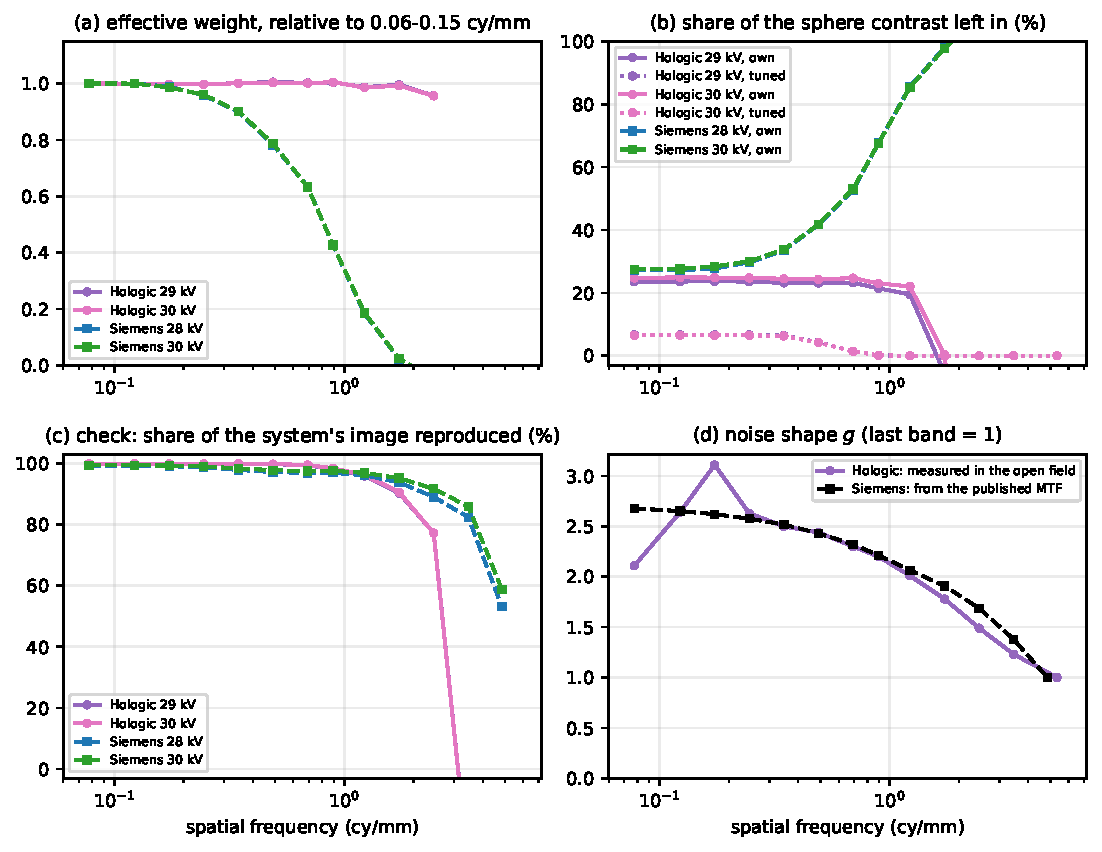
\includegraphics[width=0.95\textwidth]{hologic.pdf}
\caption{Hologic (dots, solid) against Siemens (squares, dashed), medians over the exposures. (a) Effective weight per
band relative to its value at 0.06--0.15\cymm. (b) Share of the sphere contrast left in by each system and by the
tuned recombination of the Hologic images. (c) Check: share of the system's image that our recombination at its
weighting reproduces (range shaded for Hologic). (d) Noise shape $g$: measured in the Hologic open field, and from the
published MTF for Siemens.}\label{fig:hologic}
\end{figure}

\begin{figure}[H]\centering
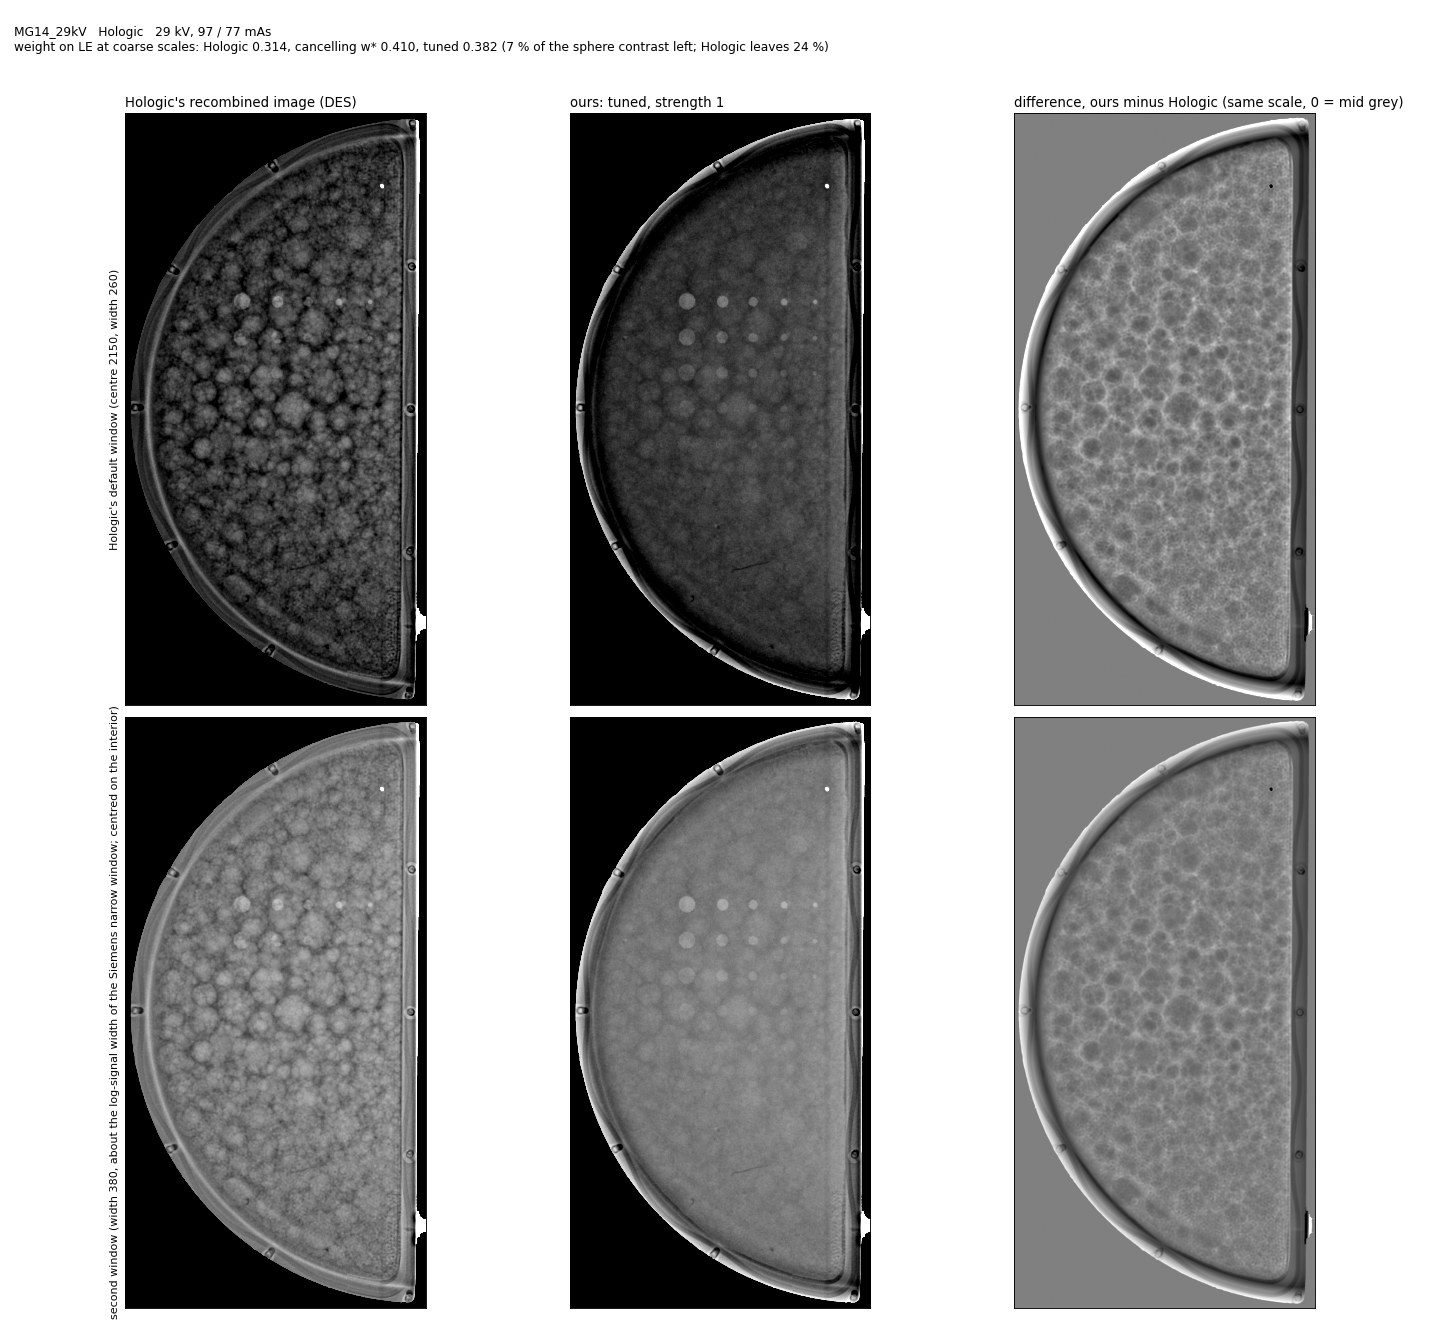
\includegraphics[width=0.93\textwidth]{comparison_hologic.jpg}
\caption{The comparison picture of one Hologic exposure (MG14, 29 kV, 61 N): Hologic's DES, the tuned image, and
their difference. Top row: Hologic's default window (centre 2150, width 260). Bottom row: width 380 centred on the
interior median.}\label{fig:hologiccomp}
\end{figure}

% =====================================================================================================================
\section{Assumptions and limits}
\begin{enumerate}
\item \textbf{Siemens' algorithm is inferred.} Sections 2 and 6 describe what the images contain. The linear model
holds in the interior and not in the outer $\approx$15 mm.
\item \textbf{Stored-value offset.} A possible offset of the LE and HE stored values is not corrected.
\item \textbf{Noise.} The highest band is taken as noise only, and the noise shape comes from a published MTF of
another unit of the same detector type, extended above 6\cymm\ by hand.
\item \textbf{Breast target.} Nine views of two patients, on another unit of the same type, at 27--28 kV; the views
differ by a factor of about five. The target is the median. It is used unchanged for 30 and 32 kV.
\item \textbf{Amount, not origin.} The target is matched in power at coarse scales. In the breasts only 1--33 \% of
it (median 14 \%) is tissue structure left by the weight; the rest is content that the LE image does not predict,
and its cause was not separated. In the phantom the same power is reached mainly with sphere structure that is left
in on purpose (Section~\ref{sec:origin}).
\item \textbf{Limits of the fade.} 0.3 and 1\cymm\ are read from the breast target. They are a choice, not a fitted
result.
\item \textbf{Siemens' LE filter $K$} in the breast target comes from an earlier fit on another unit; it agrees with
$\weff/W$ on the new unit (Fig.~\ref{fig:siemens}b).
\item \textbf{One share for the coarse bands.} The tuned image has the sphere spectrum scaled down, not a breast
spectrum. Its residual power lies inside the range of the breasts, not on their median in every band.
\item \textbf{Iodine.} The LE image also contains a (small) iodine signal, so a higher weight on LE lowers the
iodine contrast slightly. This was not quantified here.
\item \textbf{Spots.} Bright/dark pairs in single images (possibly air bubbles) are outside the model. Their ROIs
are left out of the measurement, but the spots stay in the image.
\item \textbf{Hologic: breast target.} The Siemens target is used unchanged for Hologic, because no raw Hologic breast
images exist here (Section~\ref{sec:hologictarget}). It is an assumption, not a measurement.
\item \textbf{Hologic: noise shape.} Measured in the open field, where large-scale non-quantum structure raises the lowest
bands. The effect on the left-in share is at most 0.4 percentage points.
\item \textbf{Hologic: data.} Fifteen exposures of one unit at two tube voltages, all at about the same dose. A
stored-value offset is not corrected here either; the raw LE values in the interior are 410--530 (Siemens example
exposure 540), so an offset would matter about as much as on Siemens.
\item \textbf{Use.} The tuned images are research output, not the manufacturers' output and not for diagnosis.
\end{enumerate}

% =====================================================================================================================
\section{Reference: constants, symbols, files}

\begin{table}[H]\centering\small
\caption{Fixed numbers of the script.}
\begin{tabular}{lll}
\toprule
name in the script & value & meaning \\
\midrule
\code{EDGES} & 0.06 \ldots 5.88\cymm & band edges (Table~\ref{tab:bands}) \\
\code{N} & 128 pixels & ROI size; grid step $N/2$ \\
\code{MARGIN\_MM} & 25.5 mm & ROIs lie this far inside the outline \\
footprint threshold & $0.6\times$ 99.5th percentile of HE & object outline; opening 3 iterations \\
selection limit & median $+\,3.5$ robust SD & on ln residual power, 0.1--1.0\cymm; $\le8$ passes \\
\code{BREAST['T']} & Table~\ref{tab:bands} & breast target (mm$^2$) \\
\code{MTF} & see Section~\ref{sec:noise} & detector MTF at 0--14\cymm \\
\code{FADE} & (0.3, 1.0)\cymm & share constant to 0.3, zero from 1.0 \\
share limit & 0.6 & upper limit of $\rho_0$ \\
$R^2$ limit & 0.2 & below it a band is not corrected \\
\code{F0} & 0.05\cymm & large-scale roll-off (Eq.~\ref{eq:rolloff}) \\
continuation & dilation 10 px, Gaussian 60 px & outside the object, before filtering \\
padding & 256 px, reflection & before the FFT \\
check margin & 15 mm & interior/edge zone of the check \\
\code{NARROW} & 800 grey values & narrow window of the comparison picture \\
\bottomrule
\end{tabular}
\end{table}

\begin{table}[H]\centering\small
\caption{Symbols.}
\begin{tabular}{ll}
\toprule
$\LL$, $\LH$ & log signals of the LE and HE image, $-\ln$(stored value) \\
$R$, $R_\mathrm{tuned}$ & Siemens' recombined image, the tuned image (grey values) \\
$S_{XY}(b)$ & cross-spectral density of $X$ and $Y$ in band $b$ (Eq.~\ref{eq:psd}) \\
$W$ & Siemens' weight in the header of $R$ \\
$\alpha$, $\beta$, $\weff$ & Siemens' gain, LE coefficient and effective weight, measured from $R$ (Eq.~\ref{eq:alphabeta}) \\
$K=\weff/W$ & Siemens' LE filter \\
$\ws$ & weight that cancels the background (Eq.~\ref{eq:wstar}) \\
$\gamma^2$, $C$ & coherence and cancellable power (Eq.~\ref{eq:C}) \\
$P_D(w)$ & power of $\LH-w\LL$ (Eq.~\ref{eq:PD}) \\
$g$ & shape of the quantum-noise spectrum (Eq.~\ref{eq:g}) \\
$E$ & non-noise residual of the phantom at $\ws$ (Eq.~\ref{eq:E}) \\
$T$ & breast target: structured residual under Siemens' weighting (Eq.~\ref{eq:T}) \\
$U$ & part of the breast residual that is tissue structure left by Siemens' weight (Eq.~\ref{eq:U}) \\
$\rho$, $\rho_0$, $s$ & share of the background contrast left in; its coarse-scale value; strength \\
$\wt$ & tuned weight, $\ws(1-\rho)$ \\
$c$ & correction filter (Eq.~\ref{eq:tuned}) \\
\bottomrule
\end{tabular}
\end{table}

\paragraph{Running the script.} In the folder of the measurements:
\begin{verbatim}
python3 l2_tuned_recombination.py                    # all, strength 1.0
python3 l2_tuned_recombination.py 28kV --strengths 1.0 0.5
python3 l2_tuned_recombination.py --siemens-weighting  # with the check
\end{verbatim}
{\sloppy Output: one folder \code{<kV>kV\_strength\_<s>/<session>/} with, per exposure, \code{<id>\_tuned.dcm},
\code{<id>\_comparison.png}, \code{<id>\_curves.png} and \code{<id>\_curves.csv}; a folder
\code{<kV>kV\_siemens\_weighting/} for the check; a \code{summary.csv} per folder; and all numbers in the Excel
file \code{L2\_tuned\_recombination\_numbers.xlsx} (sheets \code{tuned\_images}, \code{siemens\_weighting\_check},
\code{tuned\_curves}, \code{check\_curves}, \code{notes}).\par} The figures of this
document are made from that file, and from the Excel file of the Hologic run, by \code{make\_figures.py}, which lies
next to this document.

\paragraph{The multi-system script.} It finds Siemens and Hologic images by the manufacturer in the header, also files
without an ending. In the folder of the Hologic measurements:
{\small\begin{verbatim}
python3 ../l2_tuned_recombination_multisystem.py . --system-weighting --out .
cd ..; python3 l2_tuned_recombination_multisystem.py hologic --out hologic --strengths 2
python3 compare_systems.py      # system_comparison.xlsx, both systems
\end{verbatim}}
{\sloppy The option \code{-{}-share} sets the left-in share at strength 1 directly; use it with a separate
\code{-{}-out} folder, because results that already exist are kept. Output as above, with the main folder named \code{Hologic\_<kV>kV}, the check in
\code{Hologic\_<kV>kV\_hologic\_weighting/}, and all numbers in \code{L2\_tuned\_recombination\_multisystem\_numbers.xlsx}.
Each line of its summary also holds the acquisition data from the headers (Table~\ref{tab:acq}).
\code{hologic\_noise\_shape.py} measures the Hologic noise shape of Section~\ref{sec:hologicprofile}.\par}

\begin{table}[H]\centering\small
\caption{What depends on the system in \code{l2\_tuned\_recombination\_multisystem.py}.}\label{tab:profiles}
\setlength{\tabcolsep}{4pt}
\begin{tabular}{lll}
\toprule
 & Siemens & Hologic \\
\midrule
recombined image & image type RECOMBINED & image type SUBTRACTION (DES) \\
pairing with LE, HE & event UIDs in $R$ & HE by event UID, LE by time \\
pixel; ROI size & 0.085 mm; 128 px & 0.070 mm; 156 px (both 10.9 mm) \\
last band & 4--5.88\cymm & 4--7.14\cymm \\
noise shape $g$ & published MTF (Sec.~\ref{sec:noise}) & measured in the open field \\
weight in the header & yes (private tag) & none \\
breast target & measured (Sec.~\ref{sec:breast}) & the Siemens table, unchanged\As \\
second window of the picture & 800 grey values & 380 grey values \\
\bottomrule
\end{tabular}
\end{table}

\paragraph{Where each step is in the code.} The function names are the same in both scripts.
\code{footprint} (outline); \code{Rois} (detrend, window, spectra); \code{select} (regions left out);
\code{measure} (Eqs.~\ref{eq:wstar}, \ref{eq:C}, \ref{eq:alphabeta}, \ref{eq:E}); \code{noise\_shape}
(Eq.~\ref{eq:g}); \code{design} (Eqs.~\ref{eq:rho0}, \ref{eq:fade}); \code{Padded} (continuation, padding, filter,
Eq.~\ref{eq:rolloff}); \code{process} (Eq.~\ref{eq:tuned}, the check of Eq.~\ref{eq:check}, output). The
multi-system script adds \code{Bands} (bands, ROI size and noise shape per system) and \code{acquisition} (header
data).


\paragraph{Literature behind the method.} Table~\ref{tab:lit} lists, for each element of the method, the published
work it rests on, and what was added in this work. All references were checked against PubMed, Crossref, the
publisher or, for the white papers, the document itself (November 2026).

\begin{table}[H]\centering\footnotesize
\caption{Where the elements of the method come from.}\label{tab:lit}
\begin{tabular}{p{4.2cm}p{3.5cm}p{7.2cm}}
\toprule
element & literature & taken from it / added in this work \\
\midrule
log signal, weighted log subtraction, cancelling weight (Eqs.~\ref{eq:log}, \ref{eq:Dw}) & \cite{alvarez1976,lehmann1981,johns1985,johns1987,lewin2003,korporaal2018} & standard dual-energy and CEM physics \\
weight depends on spectrum and thickness; tissue cancellation in CEM is incomplete & \cite{carton2010,hu2017,hill2013b,knogler2016} & used to explain the header weight and the breast residual \\
ROI spectra: detrend, Hann window, averaged periodogram (Eq.~\ref{eq:psd}) & \cite{welch1967,carter1973,harris1978,zhou2011,dobbins2006,iec62220} & standard estimators; ROI size and window are our choice, not the IEC procedure \\
coherence, $\ws=S_{HL}/S_{LL}$, two-input regression per band (Eqs.~\ref{eq:wstar}, \ref{eq:C}, \ref{eq:alphabeta}) & \cite{bendat2010,carter1973} & standard estimators. Added here: measuring the manufacturer's effective weight and gain per band from its own image, and the cancelling weight of the phantom from the image pair \\
weight that minimises the background & \cite{fredenberg2010} & related: optimal weighting $\approx$ minimal anatomical noise. The least-squares estimate from the image pair is ours \\
frequency-dependent filtering in dual-energy imaging (Siemens' LE filter; our correction filter, Eq.~\ref{eq:tuned}) & \cite{macovski1983,cao1988,mccollough1989,johns1985,warp2003,richard2008,allec2013} & principle established. Siemens' LE low-pass is our measurement; it is not in the manufacturer's description \cite{korporaal2018,knogler2016} \\
anatomical noise, power law, structured vs quantum part (Eqs.~\ref{eq:PDbreast}, \ref{eq:T}) & \cite{burgess2001,heine2002,bochud1999,richard2005,hill2013a,hill2013b,mainprize2012} & the decomposition follows \cite{hill2013a}. The breast target (structured residual under the manufacturer's weighting) is ours \\
noise shape: MTF, sampling, aliasing (Eq.~\ref{eq:g}) & \cite{dobbins1995,albert2000,cunningham2000,zhao1997,zhao2003,nhsbsp} & standard model; the last band taken as noise only is an assumption. Hologic: measured in the open field (ours) \\
LE/HE motion and registration & \cite{allec2012,sistermanns2021,foroosh2002,zitova2003} & phase correlation with sub-pixel peak; the smoothed shift field is our implementation \\
content of the breast residual (Section~\ref{sec:origin}) & \cite{hill2013b,sogani2017} & iodine uptake in normal tissue and parenchymal enhancement as candidates \\
robust ROI selection & \cite{rousseeuw1993,iglewicz1993,leys2013} & standard robust statistics \\
raised-cosine fade; continuation and padding before Fourier filtering & \cite{harris1978,moisan2011,liu2008} & standard signal processing \\
sphere phantoms, texture and its residual in CEM & \cite{gang2010,cockmartin2013,cockmartin2017,cockmartin2023,contillo2016,ding2017,ikejimba2016} & motivation for tuning the phantom's residual \\
manufacturers' descriptions & \cite{korporaal2018,knogler2016,puong2007,alsheik2020,smith2014} & weighted log subtraction, border correction; no weights or filters given \\
\midrule
\multicolumn{3}{p{15.6cm}}{\emph{New in this work, no published precedent found:} the tuned image as the manufacturer's image plus a filtered LE
correction (Eq.~\ref{eq:tuned}); the left-in share matched to the breast residual (Eqs.~\ref{eq:rho0}, \ref{eq:fade}); the
check by recombining the raw images at the measured weighting (Eq.~\ref{eq:check}); applying the Siemens target to
Hologic (an assumption).} \\
\bottomrule
\end{tabular}
\end{table}

\begin{thebibliography}{99}\small
\bibitem{albert2000} Albert M, Maidment AD. Linear response theory for detectors consisting of discrete arrays. \emph{Med Phys} 2000;27(10):2417--2434. \href{https://doi.org/10.1118/1.1286592}{doi:10.1118/1.1286592}
\bibitem{allec2012} Allec N, Abbaszadeh S, Scott CC, Lewin JM, Karim KS. Including the effect of motion artifacts in noise and performance analysis of dual-energy contrast-enhanced mammography. \emph{Phys Med Biol} 2012;57(24):8405--8425. \href{https://doi.org/10.1088/0031-9155/57/24/8405}{doi:10.1088/0031-9155/57/24/8405}
\bibitem{allec2013} Allec N, Abbaszadeh S, Scott CC, Karim KS, Lewin JM. Evaluating noise reduction techniques while considering anatomical noise in dual-energy contrast-enhanced mammography. \emph{Med Phys} 2013;40(5):051904. \href{https://doi.org/10.1118/1.4799841}{doi:10.1118/1.4799841}
\bibitem{alsheik2020} Alsheik NH. \emph{Contrast enhanced digital mammography}. White paper WP-00145-EUR-EN Rev~001. Hologic Inc.; 2020.
\bibitem{alvarez1976} Alvarez RE, Macovski A. Energy-selective reconstructions in X-ray computerized tomography. \emph{Phys Med Biol} 1976;21(5):733--744. \href{https://doi.org/10.1088/0031-9155/21/5/002}{doi:10.1088/0031-9155/21/5/002}
\bibitem{bendat2010} Bendat JS, Piersol AG. \emph{Random Data: Analysis and Measurement Procedures}. 4th ed. Hoboken: Wiley; 2010 (ch.~6 single-input/output, ch.~7 multiple-input/output relationships). ISBN 978-0-470-24877-5. \href{https://doi.org/10.1002/9781118032428}{doi:10.1002/9781118032428}
\bibitem{bochud1999} Bochud FO, Valley JF, Verdun FR, Hessler C, Schnyder P. Estimation of the noisy component of anatomical backgrounds. \emph{Med Phys} 1999;26(7):1365--1370. \href{https://doi.org/10.1118/1.598632}{doi:10.1118/1.598632}
\bibitem{burgess2001} Burgess AE, Jacobson FL, Judy PF. Human observer detection experiments with mammograms and power-law noise. \emph{Med Phys} 2001;28(4):419--437. \href{https://doi.org/10.1118/1.1355308}{doi:10.1118/1.1355308}
\bibitem{cao1988} Cao Q, Brosnan T, Macovski A, Nishimura D. Least squares approach in measurement-dependent filtering for selective medical images. \emph{IEEE Trans Med Imaging} 1988;7(2):154--160. \href{https://doi.org/10.1109/42.3942}{doi:10.1109/42.3942}
\bibitem{carter1973} Carter GC, Knapp CH, Nuttall AH. Estimation of the magnitude-squared coherence function via overlapped fast Fourier transform processing. \emph{IEEE Trans Audio Electroacoust} 1973;21(4):337--344. \href{https://doi.org/10.1109/TAU.1973.1162496}{doi:10.1109/TAU.1973.1162496}
\bibitem{carton2010} Carton AK, Ullberg C, Lindman K, Acciavatti R, Francke T, Maidment AD. Optimization of a dual-energy contrast-enhanced technique for a photon-counting digital breast tomosynthesis system: I. A theoretical model. \emph{Med Phys} 2010;37(11):5896--5907. \href{https://doi.org/10.1118/1.3490556}{doi:10.1118/1.3490556}
\bibitem{cockmartin2013} Cockmartin L, Bosmans H, Marshall NW. Comparative power law analysis of structured breast phantom and patient images in digital mammography and breast tomosynthesis. \emph{Med Phys} 2013;40(8):081920. \href{https://doi.org/10.1118/1.4816309}{doi:10.1118/1.4816309}
\bibitem{cockmartin2017} Cockmartin L, Marshall NW, Zhang G, Lemmens K, Shaheen E, Van Ongeval C, et al. Design and application of a structured phantom for detection performance comparison between breast tomosynthesis and digital mammography. \emph{Phys Med Biol} 2017;62(3):758--780. \href{https://doi.org/10.1088/1361-6560/aa5407}{doi:10.1088/1361-6560/aa5407}
\bibitem{cockmartin2023} Cockmartin L, Bosmans H, Marshall NW. Investigation of test methods for QC in dual-energy based contrast-enhanced digital mammography systems: I. Iodine signal testing. \emph{Phys Med Biol} 2023;68(21):215017. \href{https://doi.org/10.1088/1361-6560/ad027d}{doi:10.1088/1361-6560/ad027d}
\bibitem{contillo2016} Contillo A, Di Domenico G, Cardarelli P, Gambaccini M, Taibi A. A novel approach to background subtraction in contrast-enhanced dual-energy digital mammography with commercially available mammography devices: Noise minimization. \emph{Med Phys} 2016;43(6):3080--3089. \href{https://doi.org/10.1118/1.4951730}{doi:10.1118/1.4951730}
\bibitem{cunningham2000} Cunningham IA. Applied linear-systems theory. In: Beutel J, Kundel HL, Van Metter RL (eds). \emph{Handbook of Medical Imaging, Vol.~1: Physics and Psychophysics}. Bellingham: SPIE Press; 2000:79--159. \href{https://doi.org/10.1117/3.832716.ch2}{doi:10.1117/3.832716.ch2}
\bibitem{ding2017} Ding H, Molloi S. Quantitative contrast-enhanced spectral mammography based on photon-counting detectors: A feasibility study. \emph{Med Phys} 2017;44(8):3939--3951. \href{https://doi.org/10.1002/mp.12296}{doi:10.1002/mp.12296}
\bibitem{dobbins1995} Dobbins JT 3rd. Effects of undersampling on the proper interpretation of modulation transfer function, noise power spectra, and noise equivalent quanta of digital imaging systems. \emph{Med Phys} 1995;22(2):171--181. \href{https://doi.org/10.1118/1.597600}{doi:10.1118/1.597600}
\bibitem{dobbins2006} Dobbins JT 3rd, Samei E, Ranger NT, Chen Y. Intercomparison of methods for image quality characterization. II. Noise power spectrum. \emph{Med Phys} 2006;33(5):1466--1475. \href{https://doi.org/10.1118/1.2188819}{doi:10.1118/1.2188819}
\bibitem{foroosh2002} Foroosh H, Zerubia JB, Berthod M. Extension of phase correlation to subpixel registration. \emph{IEEE Trans Image Process} 2002;11(3):188--200. \href{https://doi.org/10.1109/83.988953}{doi:10.1109/83.988953}
\bibitem{fredenberg2010} Fredenberg E, Hemmendorff M, Cederström B, Aslund M, Danielsson M. Contrast-enhanced spectral mammography with a photon-counting detector. \emph{Med Phys} 2010;37(5):2017--2029. \href{https://doi.org/10.1118/1.3371689}{doi:10.1118/1.3371689}
\bibitem{gang2010} Gang GJ, Tward DJ, Lee J, Siewerdsen JH. Anatomical background and generalized detectability in tomosynthesis and cone-beam CT. \emph{Med Phys} 2010;37(5):1948--1965. \href{https://doi.org/10.1118/1.3352586}{doi:10.1118/1.3352586}
\bibitem{harris1978} Harris FJ. On the use of windows for harmonic analysis with the discrete Fourier transform. \emph{Proc IEEE} 1978;66(1):51--83. \href{https://doi.org/10.1109/PROC.1978.10837}{doi:10.1109/PROC.1978.10837}
\bibitem{heine2002} Heine JJ, Velthuizen RP. Spectral analysis of full field digital mammography data. \emph{Med Phys} 2002;29(5):647--661. \href{https://doi.org/10.1118/1.1445410}{doi:10.1118/1.1445410}
\bibitem{hill2013a} Hill ML, Mainprize JG, Carton AK, Muller S, Ebrahimi M, Jong RA, et al. Anatomical noise in contrast-enhanced digital mammography. Part I. Single-energy imaging. \emph{Med Phys} 2013;40(5):051910. \href{https://doi.org/10.1118/1.4801905}{doi:10.1118/1.4801905}
\bibitem{hill2013b} Hill ML, Mainprize JG, Carton AK, Saab-Puong S, Iordache R, Muller S, et al. Anatomical noise in contrast-enhanced digital mammography. Part II. Dual-energy imaging. \emph{Med Phys} 2013;40(8):081907. \href{https://doi.org/10.1118/1.4812681}{doi:10.1118/1.4812681}
\bibitem{hu2017} Hu YH, Scaduto DA, Zhao W. Optimization of contrast-enhanced breast imaging: Analysis using a cascaded linear system model. \emph{Med Phys} 2017;44(1):43--56. \href{https://doi.org/10.1002/mp.12004}{doi:10.1002/mp.12004}
\bibitem{iec62220} IEC 62220-1-2:2007. \emph{Medical electrical equipment -- Characteristics of digital X-ray imaging devices -- Part 1-2: Determination of the detective quantum efficiency -- Detectors used in mammography}. Geneva: International Electrotechnical Commission; 2007.
\bibitem{iglewicz1993} Iglewicz B, Hoaglin DC. \emph{How to Detect and Handle Outliers}. ASQC Basic References in Quality Control, vol.~16. Milwaukee: ASQC Quality Press; 1993. ISBN 0-87389-247-X.
\bibitem{ikejimba2016} Ikejimba LC, Glick SJ, Choudhury KR, Samei E, Lo JY. Assessing task performance in FFDM, DBT, and synthetic mammography using uniform and anthropomorphic physical phantoms. \emph{Med Phys} 2016;43(10):5593. \href{https://doi.org/10.1118/1.4962475}{doi:10.1118/1.4962475}
\bibitem{johns1985} Johns PC, Yaffe MJ. Theoretical optimization of dual-energy x-ray imaging with application to mammography. \emph{Med Phys} 1985;12(3):289--296. \href{https://doi.org/10.1118/1.595766}{doi:10.1118/1.595766}
\bibitem{johns1987} Johns PC, Yaffe MJ. X-ray characterisation of normal and neoplastic breast tissues. \emph{Phys Med Biol} 1987;32(6):675--695. \href{https://doi.org/10.1088/0031-9155/32/6/002}{doi:10.1088/0031-9155/32/6/002}
\bibitem{knogler2016} Knogler T, Homolka P, Hörnig M, Leithner R, Langs G, Waitzbauer M, et al. Contrast-enhanced dual energy mammography with a novel anode/filter combination and artifact reduction: a feasibility study. \emph{Eur Radiol} 2016;26(6):1575--1581. \href{https://doi.org/10.1007/s00330-015-4007-6}{doi:10.1007/s00330-015-4007-6}
\bibitem{korporaal2018} Korporaal JG, H\"ornig MD, Mertelmeier T, Hebecker A. \emph{Titanium Contrast-Enhanced Mammography (TiCEM): expand your diagnostic insights}. White paper. Erlangen: Siemens Healthcare GmbH; 2018 (no.\ 6323 0718).
\bibitem{lehmann1981} Lehmann LA, Alvarez RE, Macovski A, Brody WR, Pelc NJ, Riederer SJ, et al. Generalized image combinations in dual KVP digital radiography. \emph{Med Phys} 1981;8(5):659--667. \href{https://doi.org/10.1118/1.595025}{doi:10.1118/1.595025}
\bibitem{lewin2003} Lewin JM, Isaacs PK, Vance V, Larke FJ. Dual-energy contrast-enhanced digital subtraction mammography: feasibility. \emph{Radiology} 2003;229(1):261--268. \href{https://doi.org/10.1148/radiol.2291021276}{doi:10.1148/radiol.2291021276}
\bibitem{leys2013} Leys C, Ley C, Klein O, Bernard P, Licata L. Detecting outliers: do not use standard deviation around the mean, use absolute deviation around the median. \emph{J Exp Soc Psychol} 2013;49(4):764--766. \href{https://doi.org/10.1016/j.jesp.2013.03.013}{doi:10.1016/j.jesp.2013.03.013}
\bibitem{liu2008} Liu R, Jia J. Reducing boundary artifacts in image deconvolution. In: \emph{Proc.\ 15th IEEE International Conference on Image Processing (ICIP 2008)}; 2008:505--508. \href{https://doi.org/10.1109/ICIP.2008.4711802}{doi:10.1109/ICIP.2008.4711802}
\bibitem{macovski1983} Macovski A, Nishimura DG, Doost-Hoseini A, Brody WR. Measurement-Dependent Filtering: A Novel Approach to Improved SNR. \emph{IEEE Trans Med Imaging} 1983;2(3):122--127. \href{https://doi.org/10.1109/TMI.1983.4307625}{doi:10.1109/TMI.1983.4307625}
\bibitem{mainprize2012} Mainprize JG, Tyson AH, Yaffe MJ. The relationship between anatomic noise and volumetric breast density for digital mammography. \emph{Med Phys} 2012;39(8):4660--4668. \href{https://doi.org/10.1118/1.4736422}{doi:10.1118/1.4736422}
\bibitem{mccollough1989} McCollough CH, Van Lysel MS, Peppler WW, Mistretta CA. A correlated noise reduction algorithm for dual-energy digital subtraction angiography. \emph{Med Phys} 1989;16(6):873--880. \href{https://doi.org/10.1118/1.596436}{doi:10.1118/1.596436}
\bibitem{moisan2011} Moisan L. Periodic plus smooth image decomposition. \emph{J Math Imaging Vis} 2011;39(2):161--179. \href{https://doi.org/10.1007/s10851-010-0227-1}{doi:10.1007/s10851-010-0227-1}
\bibitem{nhsbsp} NHS Breast Screening Programme. \emph{Technical evaluation of Siemens Revelation digital breast tomosynthesis system.} Public Health England / NCCPM, March 2019, Table~10 (MTF, measured on another unit).
\bibitem{puong2007} Puong S, Bouchevreau X, Patoureaux F, Iordache R, Muller S. Dual-energy contrast enhanced digital mammography using a new approach for breast tissue canceling. \emph{Proc SPIE} 2007;6510:65102H. \href{https://doi.org/10.1117/12.710133}{doi:10.1117/12.710133}
\bibitem{richard2005} Richard S, Siewerdsen JH, Jaffray DA, Moseley DJ, Bakhtiar B. Generalized DQE analysis of radiographic and dual-energy imaging using flat-panel detectors. \emph{Med Phys} 2005;32(5):1397--1413. \href{https://doi.org/10.1118/1.1901203}{doi:10.1118/1.1901203}
\bibitem{richard2008} Richard S, Siewerdsen JH. Cascaded systems analysis of noise reduction algorithms in dual-energy imaging. \emph{Med Phys} 2008;35(2):586--601. \href{https://doi.org/10.1118/1.2826556}{doi:10.1118/1.2826556}
\bibitem{rousseeuw1993} Rousseeuw PJ, Croux C. Alternatives to the median absolute deviation. \emph{J Am Stat Assoc} 1993;88(424):1273--1283. \href{https://doi.org/10.1080/01621459.1993.10476408}{doi:10.1080/01621459.1993.10476408}
\bibitem{sistermanns2021} Sistermanns M, Kowall B, Hörnig M, Beiderwellen K, Uhlenbrock D. Motion Artifact Reduction in Contrast-Enhanced Dual-Energy Mammography -- a multireader Study about the Effect of Nonrigid Registration as Motion Correction on Image Quality. \emph{R\"oFo} 2021;193(10):1183--1188. \href{https://doi.org/10.1055/a-1388-7712}{doi:10.1055/a-1388-7712}
\bibitem{smith2014} Smith A. \emph{The principles of contrast mammography}. White paper WP-00084-001. Hologic Inc.; 2014.
\bibitem{sogani2017} Sogani J, Morris EA, Kaplan JB, D'Alessio D, Goldman D, Moskowitz CS, et al. Comparison of Background Parenchymal Enhancement at Contrast-enhanced Spectral Mammography and Breast MR Imaging. \emph{Radiology} 2017;282(1):63--73. \href{https://doi.org/10.1148/radiol.2016160284}{doi:10.1148/radiol.2016160284}
\bibitem{warp2003} Warp RJ, Dobbins JT 3rd. Quantitative evaluation of noise reduction strategies in dual-energy imaging. \emph{Med Phys} 2003;30(2):190--198. \href{https://doi.org/10.1118/1.1538232}{doi:10.1118/1.1538232}
\bibitem{welch1967} Welch PD. The use of fast Fourier transform for the estimation of power spectra: a method based on time averaging over short, modified periodograms. \emph{IEEE Trans Audio Electroacoust} 1967;15(2):70--73. \href{https://doi.org/10.1109/TAU.1967.1161901}{doi:10.1109/TAU.1967.1161901}
\bibitem{zhao1997} Zhao W, Rowlands JA. Digital radiology using active matrix readout of amorphous selenium: theoretical analysis of detective quantum efficiency. \emph{Med Phys} 1997;24(12):1819--1833. \href{https://doi.org/10.1118/1.598097}{doi:10.1118/1.598097}
\bibitem{zhao2003} Zhao W, Ji WG, Debrie A, Rowlands JA. Imaging performance of amorphous selenium based flat-panel detectors for digital mammography: characterization of a small area prototype detector. \emph{Med Phys} 2003;30(2):254--263. \href{https://doi.org/10.1118/1.1538233}{doi:10.1118/1.1538233}
\bibitem{zhou2011} Zhou Z, Gao F, Zhao H, Zhang L. Techniques to improve the accuracy of noise power spectrum measurements in digital x-ray imaging based on background trends removal. \emph{Med Phys} 2011;38(3):1600--1610. \href{https://doi.org/10.1118/1.3556566}{doi:10.1118/1.3556566}
\bibitem{zitova2003} Zitov\'a B, Flusser J. Image registration methods: a survey. \emph{Image Vis Comput} 2003;21(11):977--1000. \href{https://doi.org/10.1016/S0262-8856(03)00137-9}{doi:10.1016/S0262-8856(03)00137-9}
\end{thebibliography}

\end{document}
